\chapter{Demonstrative Experiments}
\label{chapter:demonstrative-experiments}

This chapter presents two demonstrative simulation experiments done on the Cavium OCTEON II CN6880 PSE model. The goal of the experiments is to demonstrate how the queue types, priorities, and coremasking affect the scheduler, and hence the packet throughput and latency. At the same time, it validates the PSE's implemented plugin-code functionality and the CN6880 model.

\section{Experiment Setup}
\label{sec:experiment-setup}

Both experiments are run on the hardware model represented in figure~\ref{fig:experiment-hardware}. The model consists of six active resources. The PKI and PKO units are consumed by the input and output phases of the packet flow, respectively. Each 32 processing cores have a L1 cache associated with it, and the L2 cache and RAM are shared between the cores. The cores are served as first come first serve basis, as the scheduling logic is taken care of in the SSO unit.

\begin{figure}[]
  \begin{center}
    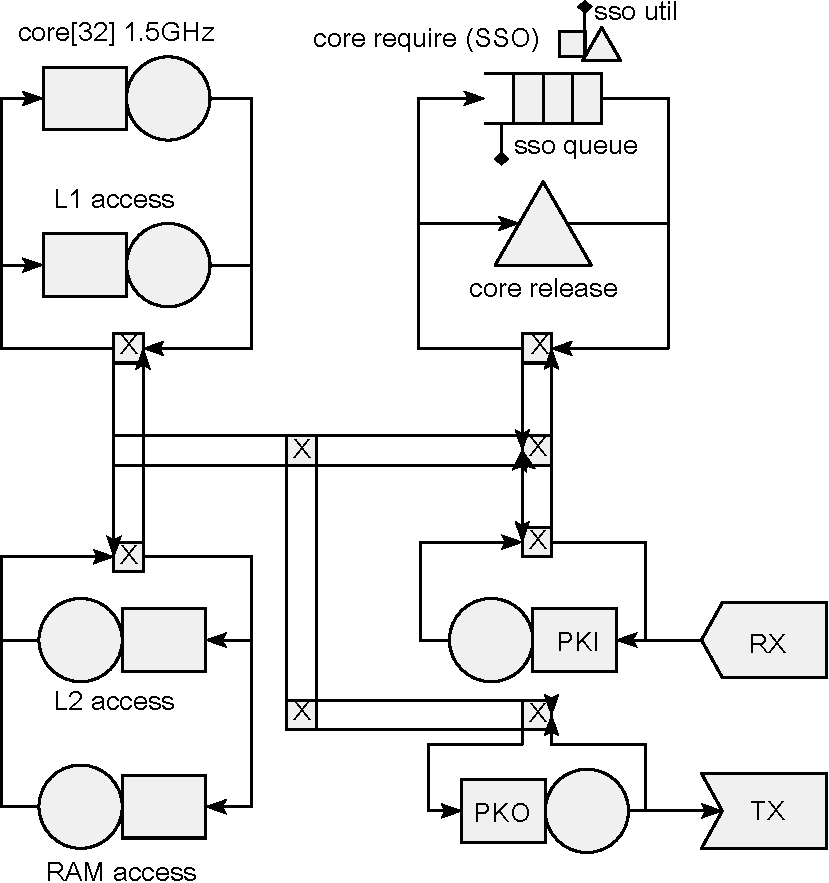
\includegraphics[width=0.6\textwidth]{images/pse-models/experiment-hardware.pdf}
    \caption{Resource provision model (hardware) used in the experiments. The model represents the Cavium Octeon CN6880 network processing unit.}
    \label{fig:experiment-hardware}
  \end{center}
\end{figure}

The SSO unit uses the custom scheduling functions presented in the section~\ref{sec:custom-scheduler-functions}, enabling the use of atomicity, queue priorities, and coremasks. The core release is a typical relase node referring to the SSO unit.

The same high level software model is used for the both experiments, as seen in the figures~\ref{fig:exp1-software} and~\ref{fig:exp2-software}. The \emph{Packet Input} and \emph{Packet Output} nodes consume the PKI and PKO units as discussed in the section~\ref{sec:characteristic-measurements}, delaying the packets relative to their size, according to the equation~\ref{eq:1}. The workload and packet process submodels are unique for both experiments.

We gather two different metrics of the system. First, we are interested in the core utilization and queue lengths for each processing step. These are measured by the probes attached to the SSO unit as shown in hardware model in figure~\ref{fig:experiment-hardware}. Secondly, we are interested in the packet latencies. They are measured by calculating the time difference between the \emph{out probe} and the \emph{in probe} (figures~\ref{fig:exp1-software} and~\ref{fig:exp2-software}) for each packet. All the probes write absolute traces of the packets.

\section{Experiment 1: Global Queue Interrelations}
The first experiment consists of two different simulations and measurements. We will first demonstrate a packet processing application, whose throughput is limited due to the bottleneck occurring from a slow atomic processing. The application is then modified, extracting part of the atomic execution object into parallel, thus breaking the bottleneck.

The workload model consists of a single packet stream, which is generated from a two level workload model, presented at the top in figure~\ref{fig:exp1-software}. The \emph{TRAFFIC GENERATOR} node triggers its child node with interval $RNS\_random\_uniform(5*10^{-5}, 15*10^{-5})$ seconds, and lifetime of 0.05 seconds. The child node creates 512B packets with interval $5.1~*~10^{-8}~*~RNS\_random\_lognormal(-10, 0.9)$ seconds for $4*10^{-5}$ seconds.

The two different applications used in the experiment are shown in the software model after the \emph{select app}-node. The lower and upper application are referred as \emph{application 1} and \emph{application 2}, respectively. The application selection is done in the workload model by the \emph{AppId} attribute.

Application 1 consists of two processing steps, both consuming CPU and memory for the range of 5000 clock cycles. The first step consists of parallel, priority 2 queue (A), and the second one is done atomically with priority 1 queue (B). Application 2 is a modified version of the first packet processing application, where the second processing step is split into parallel and atomic steps. The release nodes are omitted from the software model for clarity.

\begin{figure}[]
  \begin{center}
    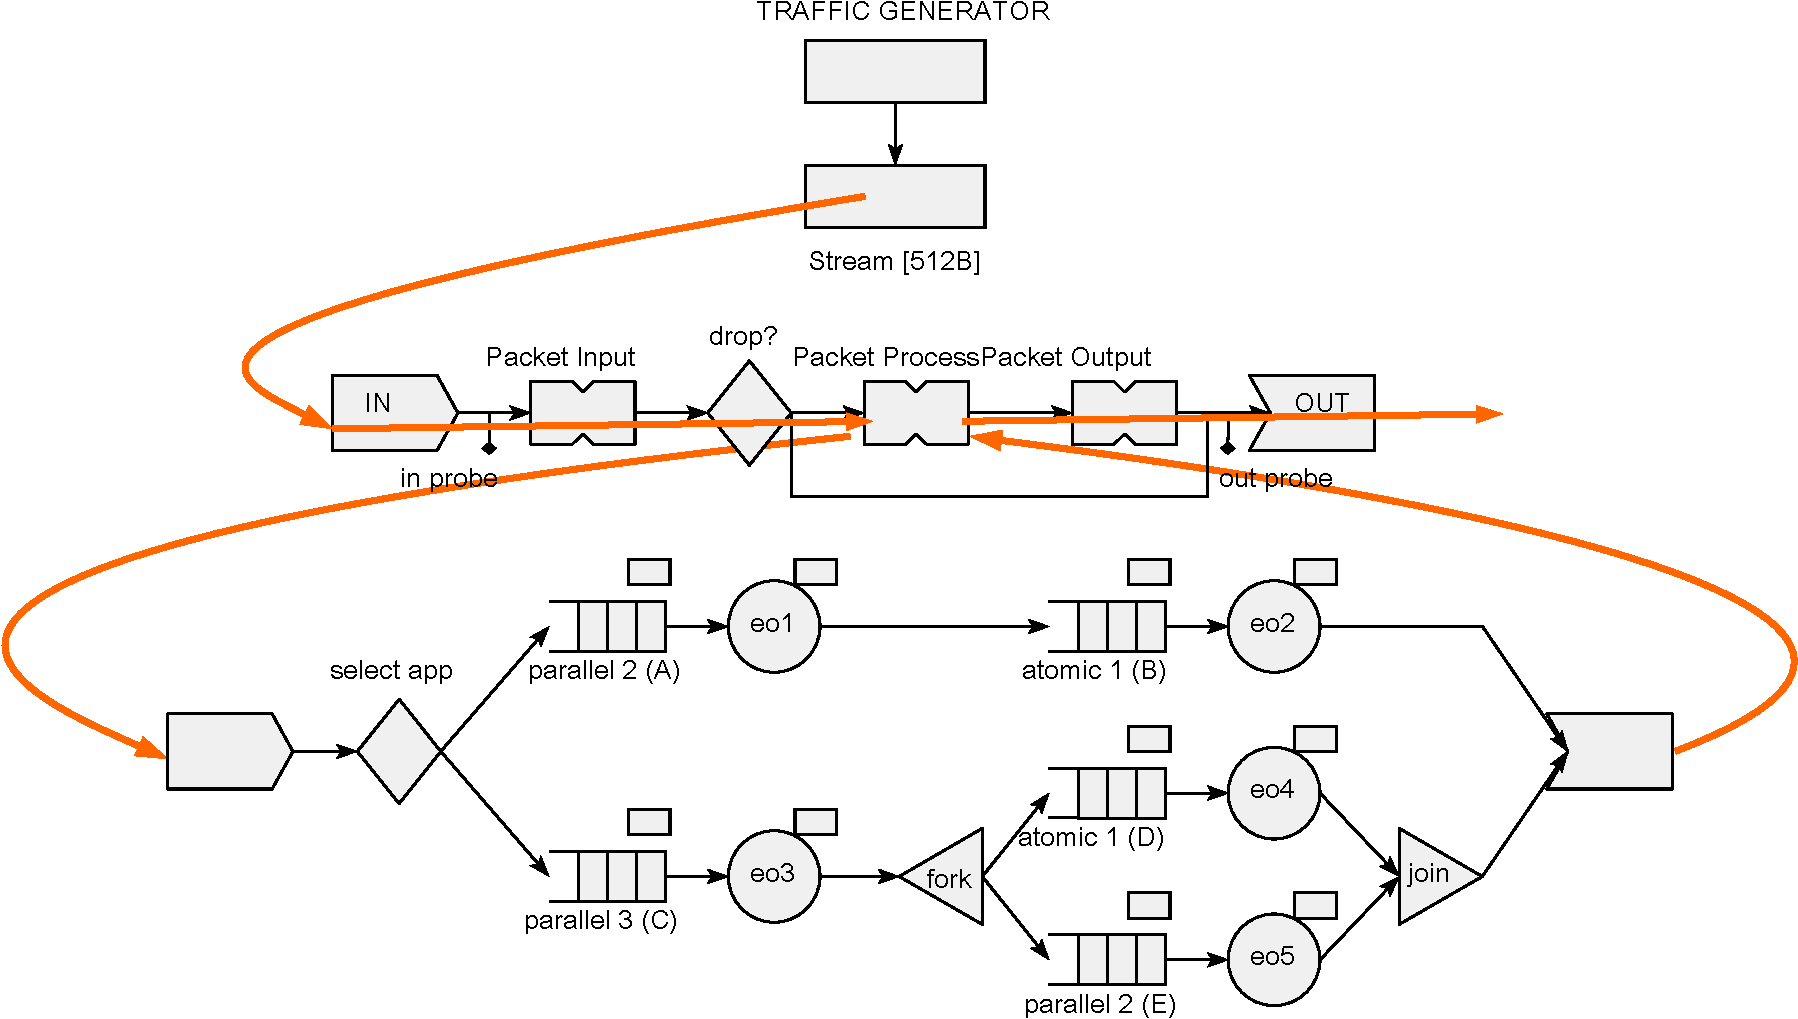
\includegraphics[width=\textwidth]{images/pse-models/exp1-software.pdf}
    \caption{Workload and resource usage (software) models used in the first experiment. The atomic queue in the upper application (application 1) produces a bottleneck to the system. The application 2 below removes this bottleneck by extracting part of the processing into parallel.}
    \label{fig:exp1-software}
  \end{center}
\end{figure}

\subsection{Simulation Results}
\label{sec:exp1-simulation-results}
The system was simulated twice, using both applications separately, and the data from the probes were post-processed. We grouped the number of tasks in the SSO/core queue, by the processing step.

Figures~\ref{fig:app1-queue2} and~\ref{fig:app1-latency} present the data from the first simulation using the packet processing application 1. Figure~\ref{fig:app1-queue2} describes the number of tasks in the SSO/core queue, that are from the atomic resource usage queue, with respect to simulation time. The corresponding graph for the first queue is omitted, as none of that tasks from it end up in the waiting queue. Figure~\ref{fig:app1-latency} presents the latency of each packet through the whole system.

\begin{figure}[]
  \begin{center}
    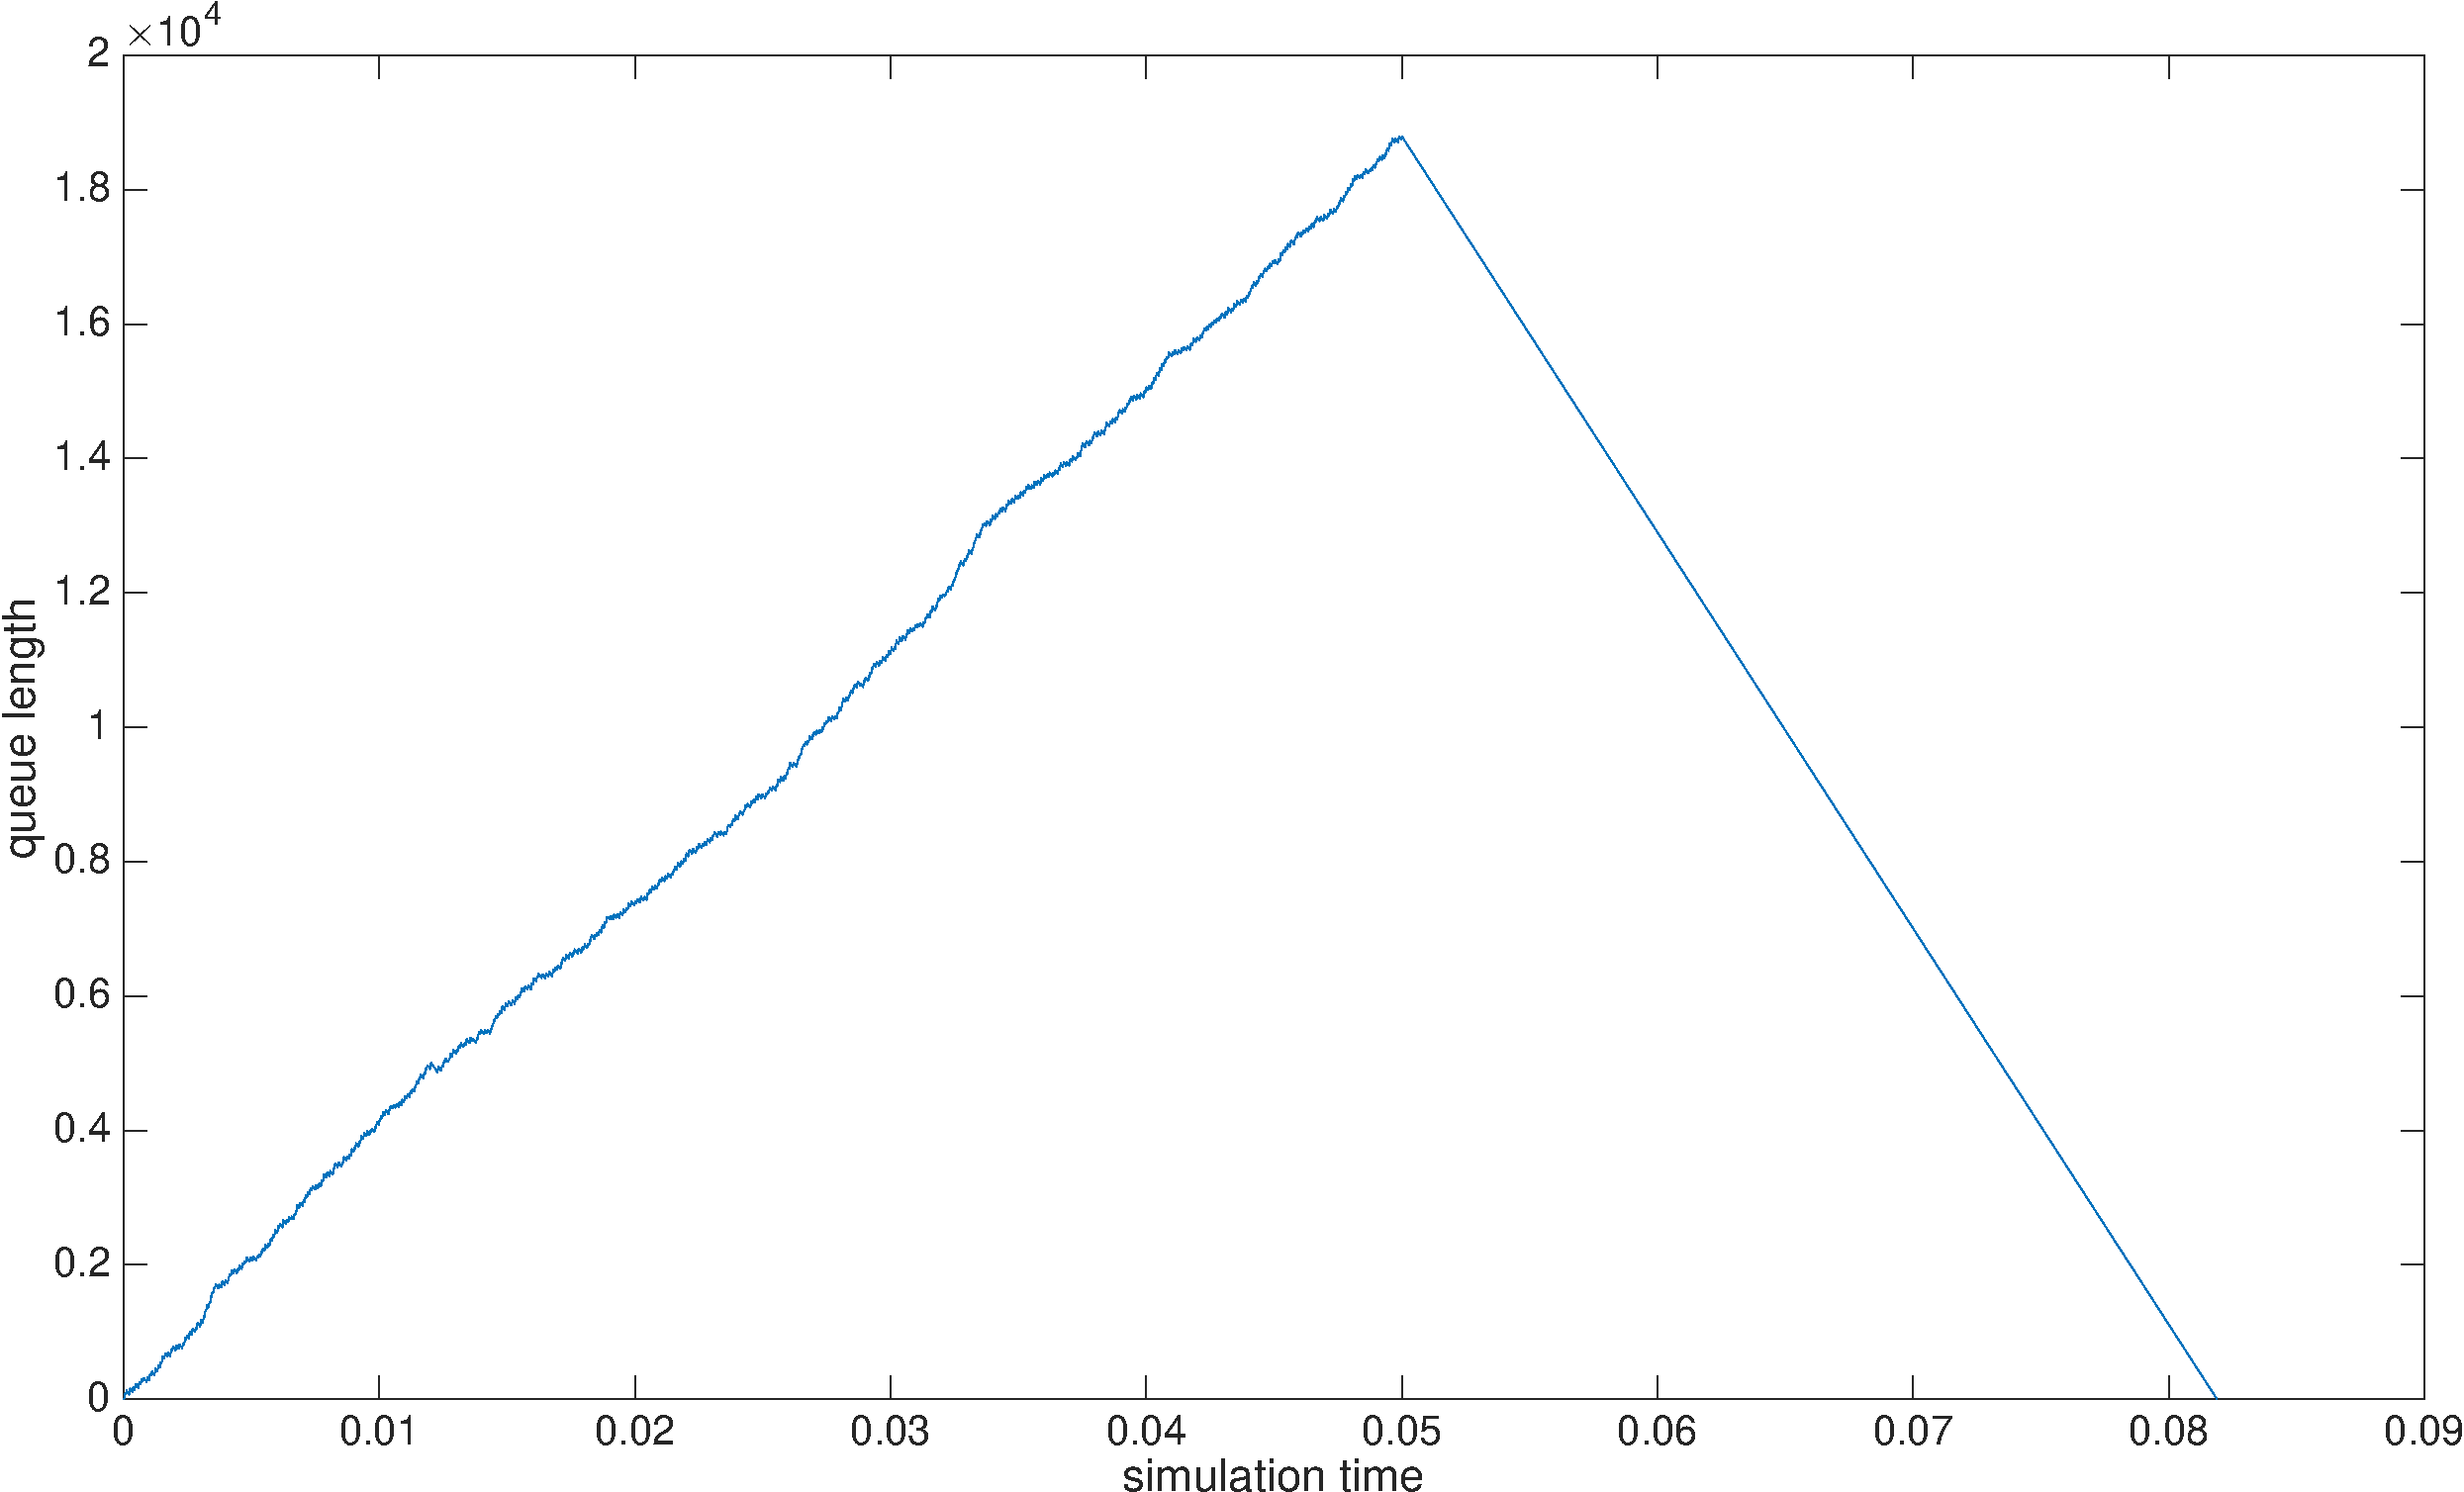
\includegraphics[width=\textwidth]{images/experiment/app1-queue2.pdf}
    \caption{Application 1: The number of tasks in the SSO/core queue, with respect to simulation time, from the second resource usage queue.}
    \label{fig:app1-queue2}
  \end{center}
\end{figure}

\begin{figure}[]
  \begin{center}
    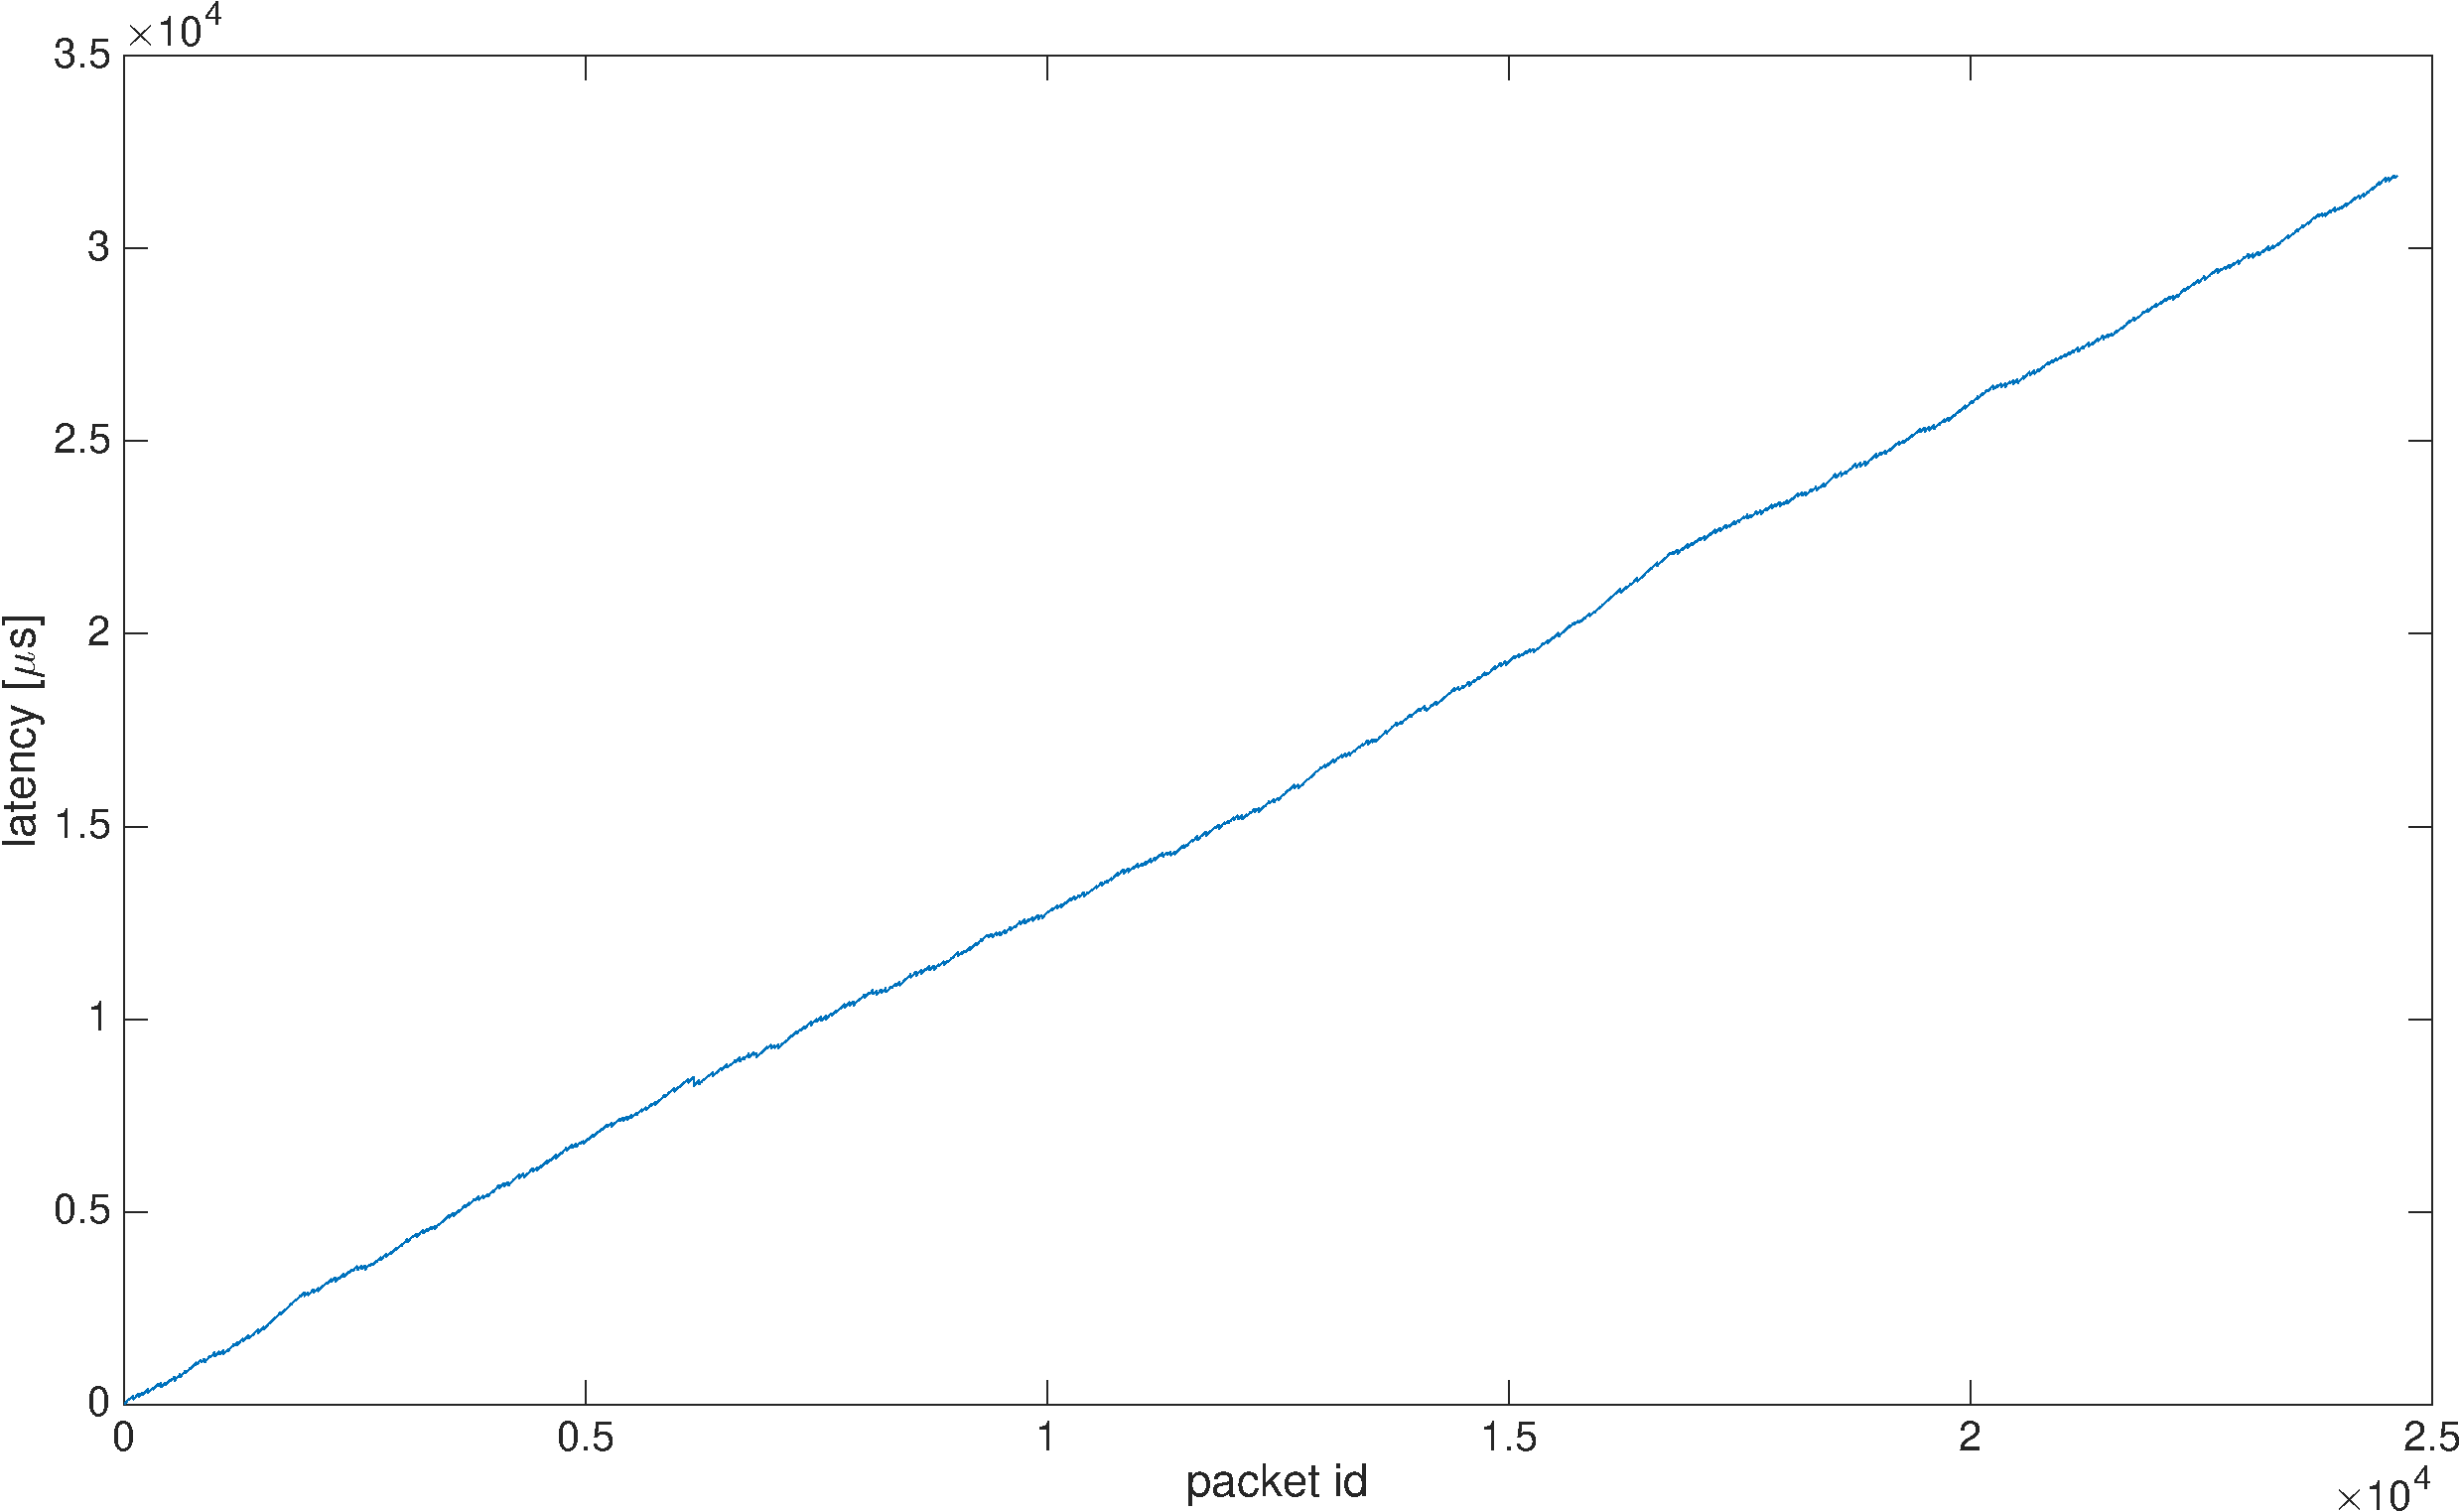
\includegraphics[width=\textwidth]{images/experiment/app1-latency.pdf}
    \caption{Application 1: Latency of the packets through the system.}
    \label{fig:app1-latency}
  \end{center}
\end{figure}

As shown in the figures, the second processing step of application 1 produces a bottleneck to the system. The processing in the second execution object is so heavy that the tasks accumulate into the waiting queue, and thus the packet latency keeps growing until the workload ceases.

The second application modifies the system by parallelizing part of the atomic processing. Figures~\ref{fig:app2-queue2} and~\ref{fig:app2-latency} present the data from the second application simulation. Figure~\ref{fig:app2-queue2} shows the number of tasks in the SSO/core queue, that are from the atomic resource usage queue, with respect to simulation time. Figure~\ref{fig:app2-latency} presents the latency of the packets through the whole system. Neither of the parallel queues have tasks in the waiting queue of the SSO/core during the simulation.

\begin{figure}[]
  \begin{center}
    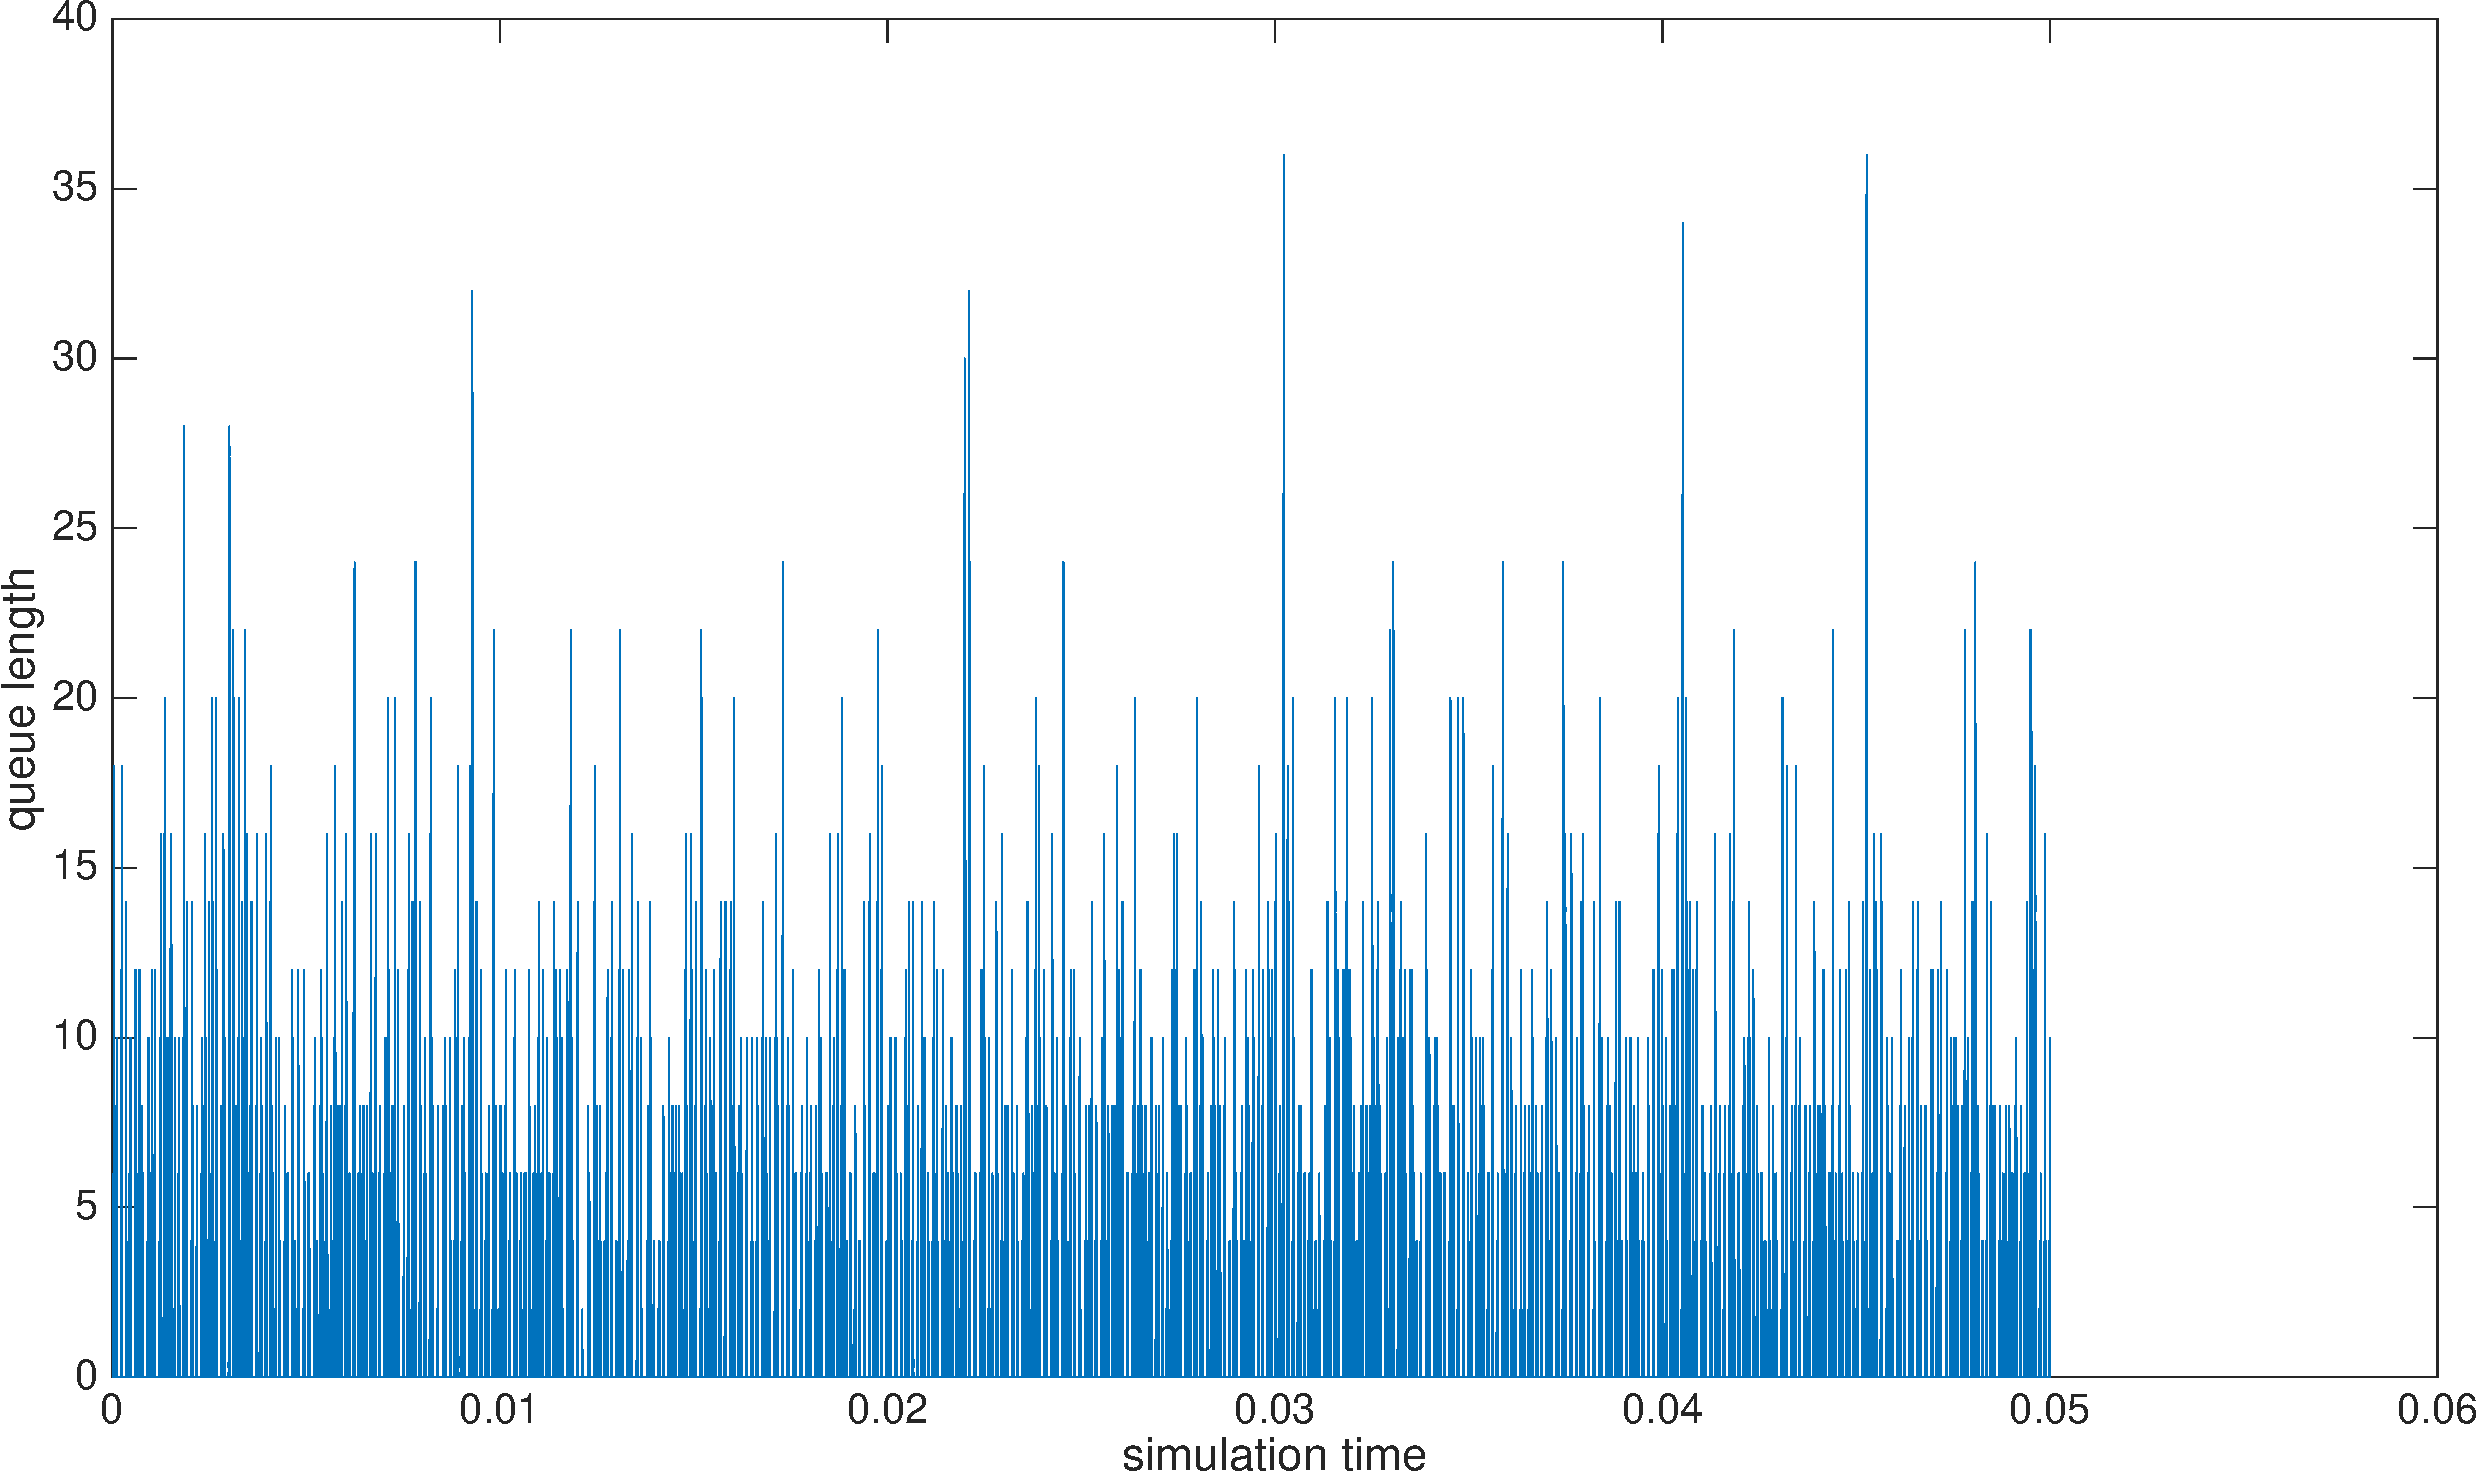
\includegraphics[width=\textwidth]{images/experiment/app2-queue2.pdf}
    \caption{Application 2: The number of tasks in the SSO/core queue, from the second resource usage queue.}
    \label{fig:app2-queue2}
  \end{center}
\end{figure}

\begin{figure}[]
  \begin{center}
    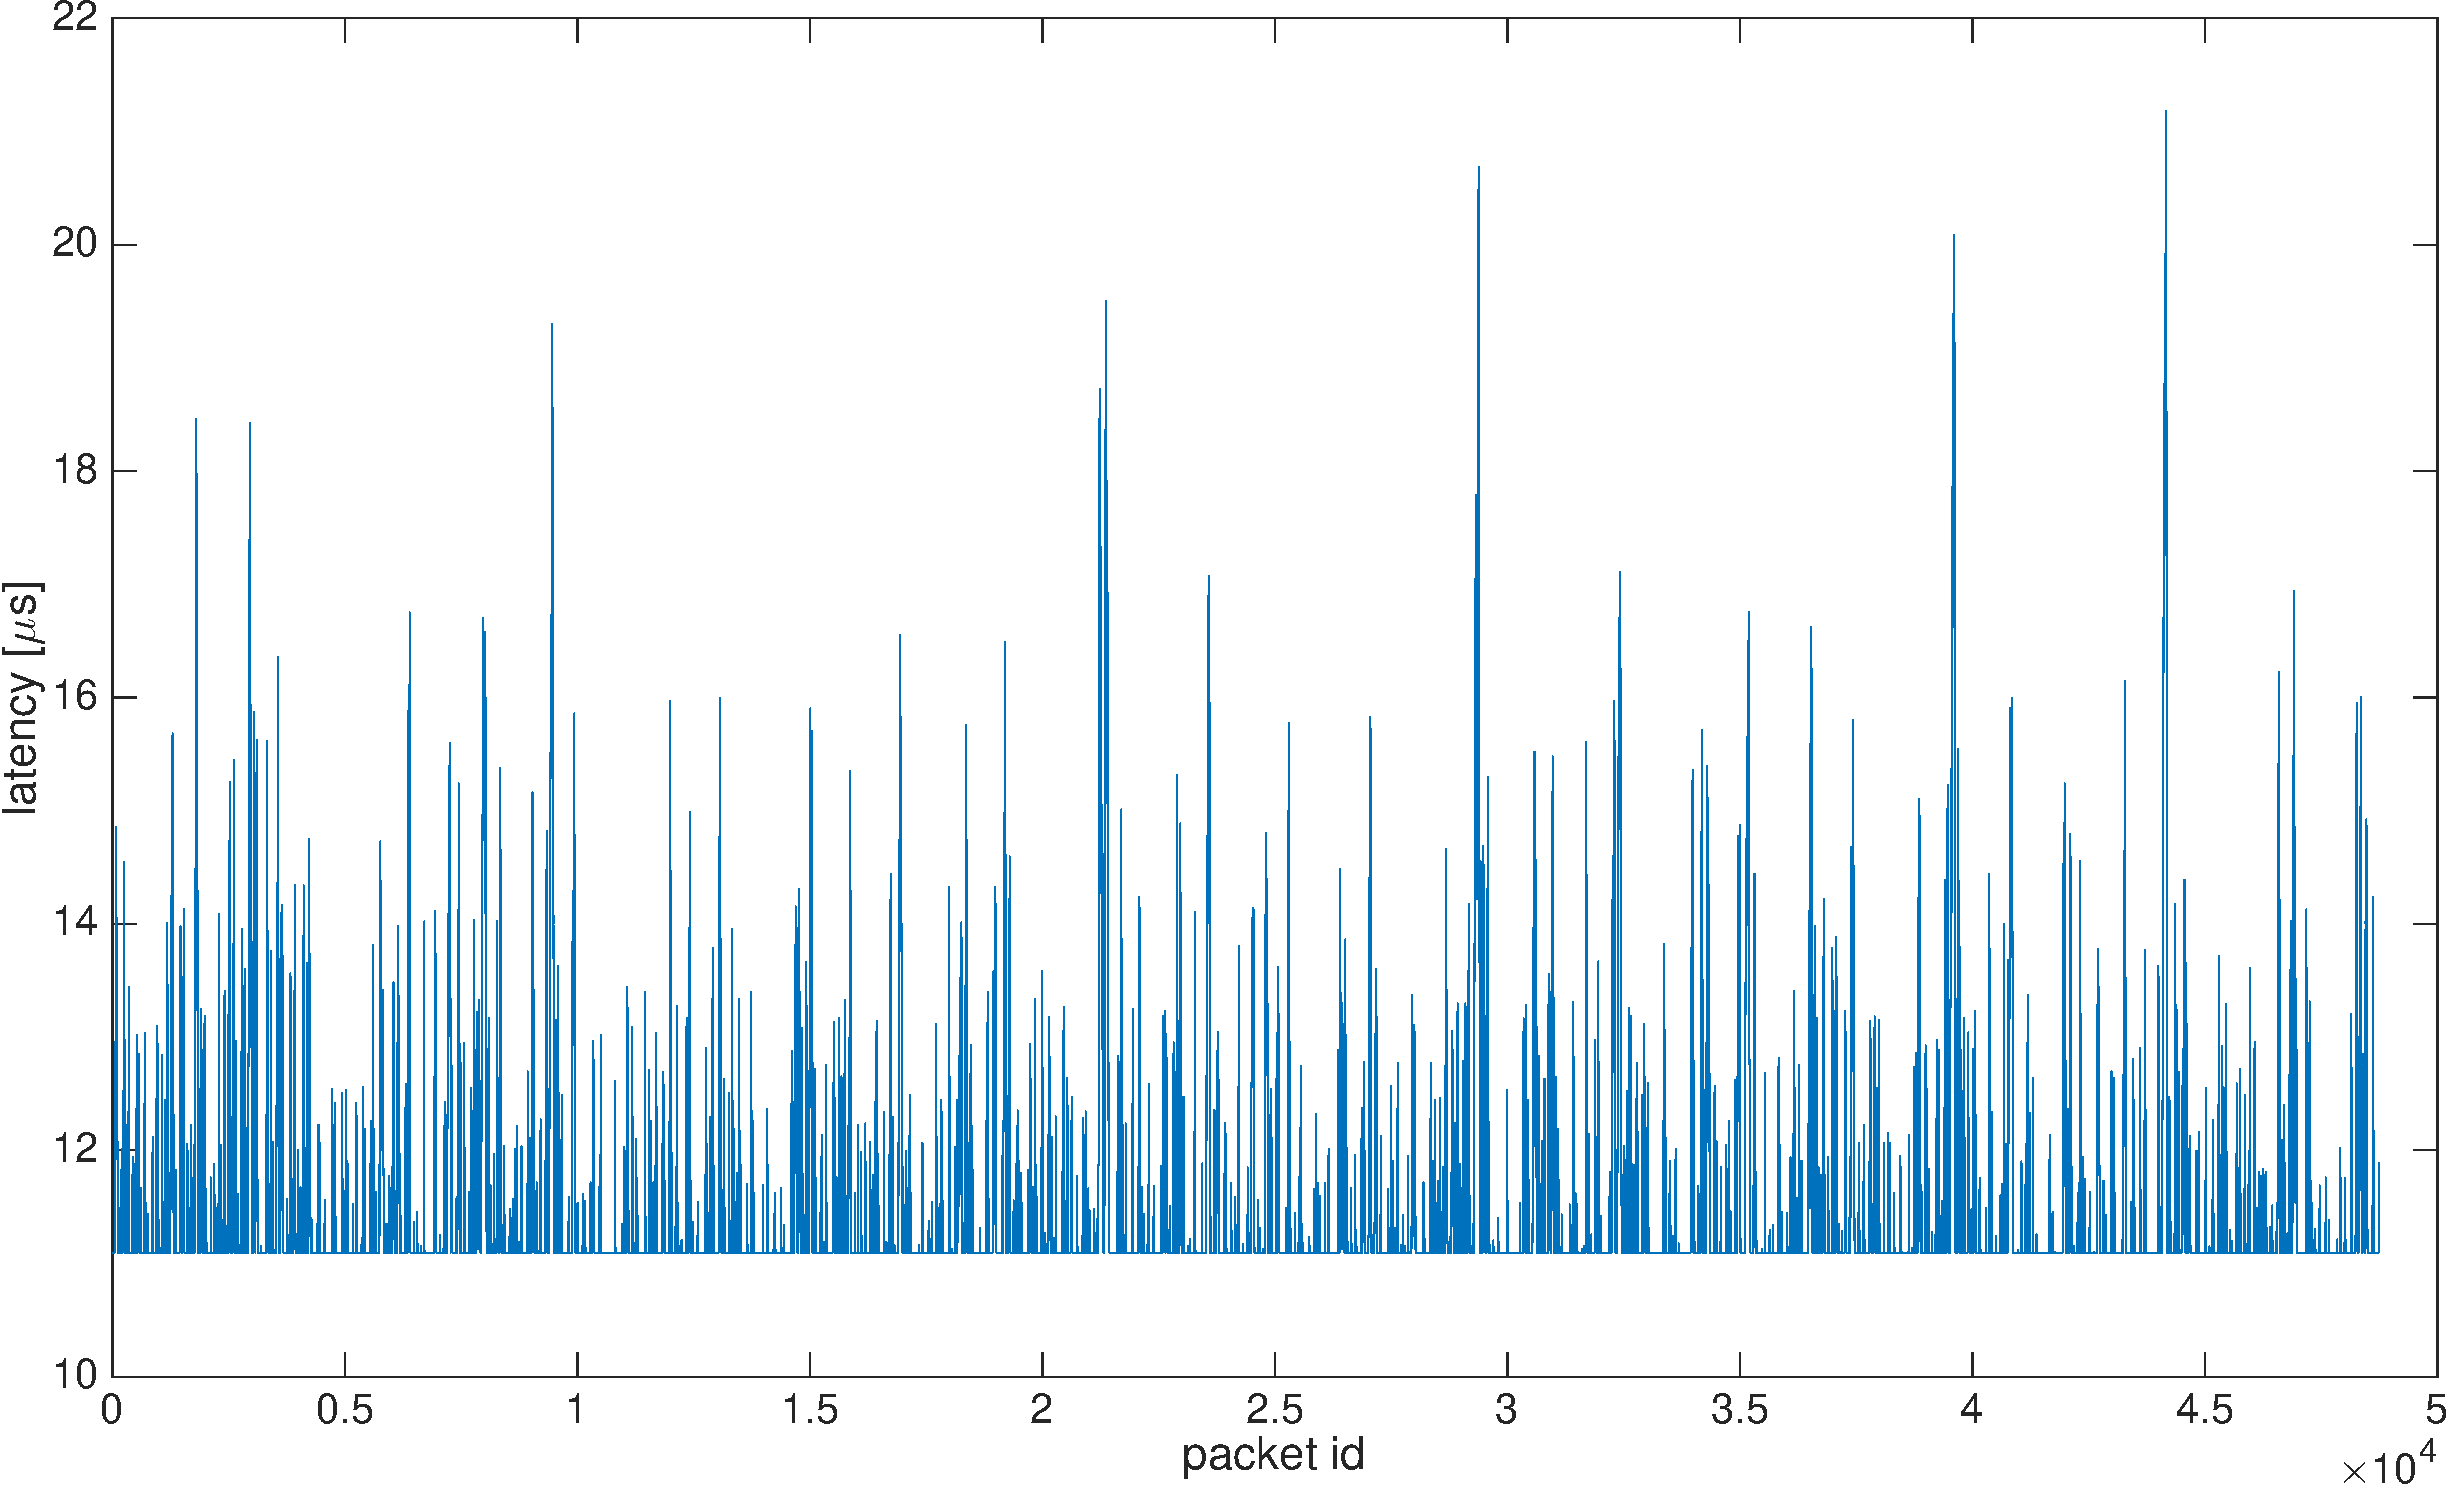
\includegraphics[width=\textwidth]{images/experiment/app2-latency.pdf}
    \caption{Application 2: Latency of the packets through the system.}
    \label{fig:app2-latency}
  \end{center}
\end{figure}

As the shown in the figures, the second application removes the bottleneck from the system. The latencies stay within 22$\mu$s, and the reducing the queue length below 40 over the whole simulation period.

\section{Experiment 2: Queue Coremasks}
% app1 heavy
% app2 light

The second experiment demonstrates the packet flow control via queue coremasks. The experiment consists of two packet flows and dedicated application processing them, as presented in figure~\ref{fig:exp2-software}. The first packet stream (presented as orange), presents a higher OSI-level application data, such as video stream, that is processed on a heavy execution object. The second stream (presented as blue), on the other hand, consists of packets whose processing is done on fast processing application with strict latency requirements.

The \emph{TRAFFIC GENERATOR} node triggers its child nodes with interval $RNS\_random\_uniform(5*10^{-5}, 15*10^{-5})$ seconds, and lifetime of 0.05 seconds. Stream 1 and Stream 2 create 512B packets with interval $6.1*10^{-7}~*~RNS\_lognormal(-10, 0.9)$ and $10^{-6}~*~RNS\_lognormal(5, 10)$ seconds for $4*10^{-5}$ and $10^{-5}$ seconds, respectively. The heavy application consumes the CPU and memory for a total of about 50000 cycles per 512B packet, while the light application packets are processed for tenth of that, in 4500 cycles.

We will again perform two different simulations and measurements. The first one is carried out by allowing the heavy application to be processed on all the 32 processing cores. Despite the light flow being processed on higher priority queue, the processing of the heavy flow has an effect to the worst case latency of the light flow packets. This happens due to the run-to-completion model of the cores, where light flow packets may have to queue for a core while the heavy tasks finish. In the seacond simulation, the heavy application processing is limited to 30 cores, dedicating two cores for the light application.

\begin{figure}[]
  \begin{center}
    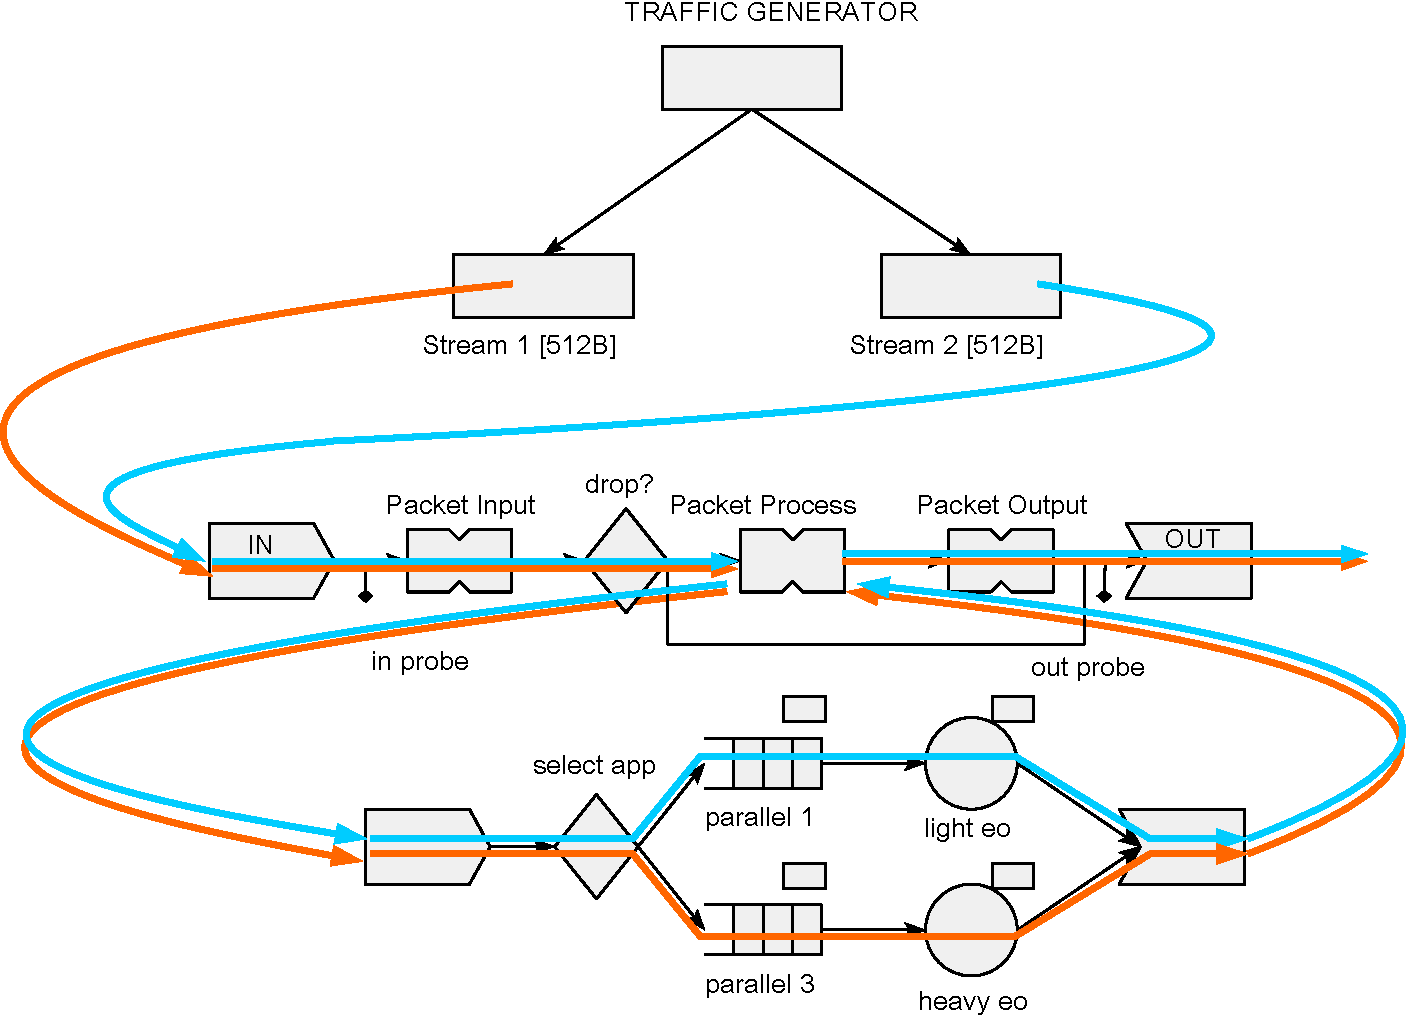
\includegraphics[width=\textwidth]{images/pse-models/exp2-software.pdf}
    \caption{TODO}
    \label{fig:exp2-software}
  \end{center}
\end{figure}

\subsection{Simulation Results}
\label{sec:exp2-simulation-results}

The system was simulated twice, once without limiting the heavy application processing cores, and once with limited coremask. The data from the probes were post-processed.

Figures~\ref{fig:exp2-app1-no-coremask-latency} and~\ref{fig:exp2-app2-no-coremask-latency} present the data from the simulation without coremask, for the heavy and light flow, respectively. The latency of the heavy flow packets is between 80$\mu$s and 340$\mu$s throughout the simulation. As shown in the figure~\ref{fig:exp2-app2-no-coremask-latency}, the light flow packets can be processed in 8$\mu$s at best. However, in the worst case, when all the cores are processing heavy flow packets, the light flow packet latency is almost ten-fold, 61$\mu$s. The throughput of the heavy application is 0.214GBps.

\begin{figure}[]
  \begin{center}
    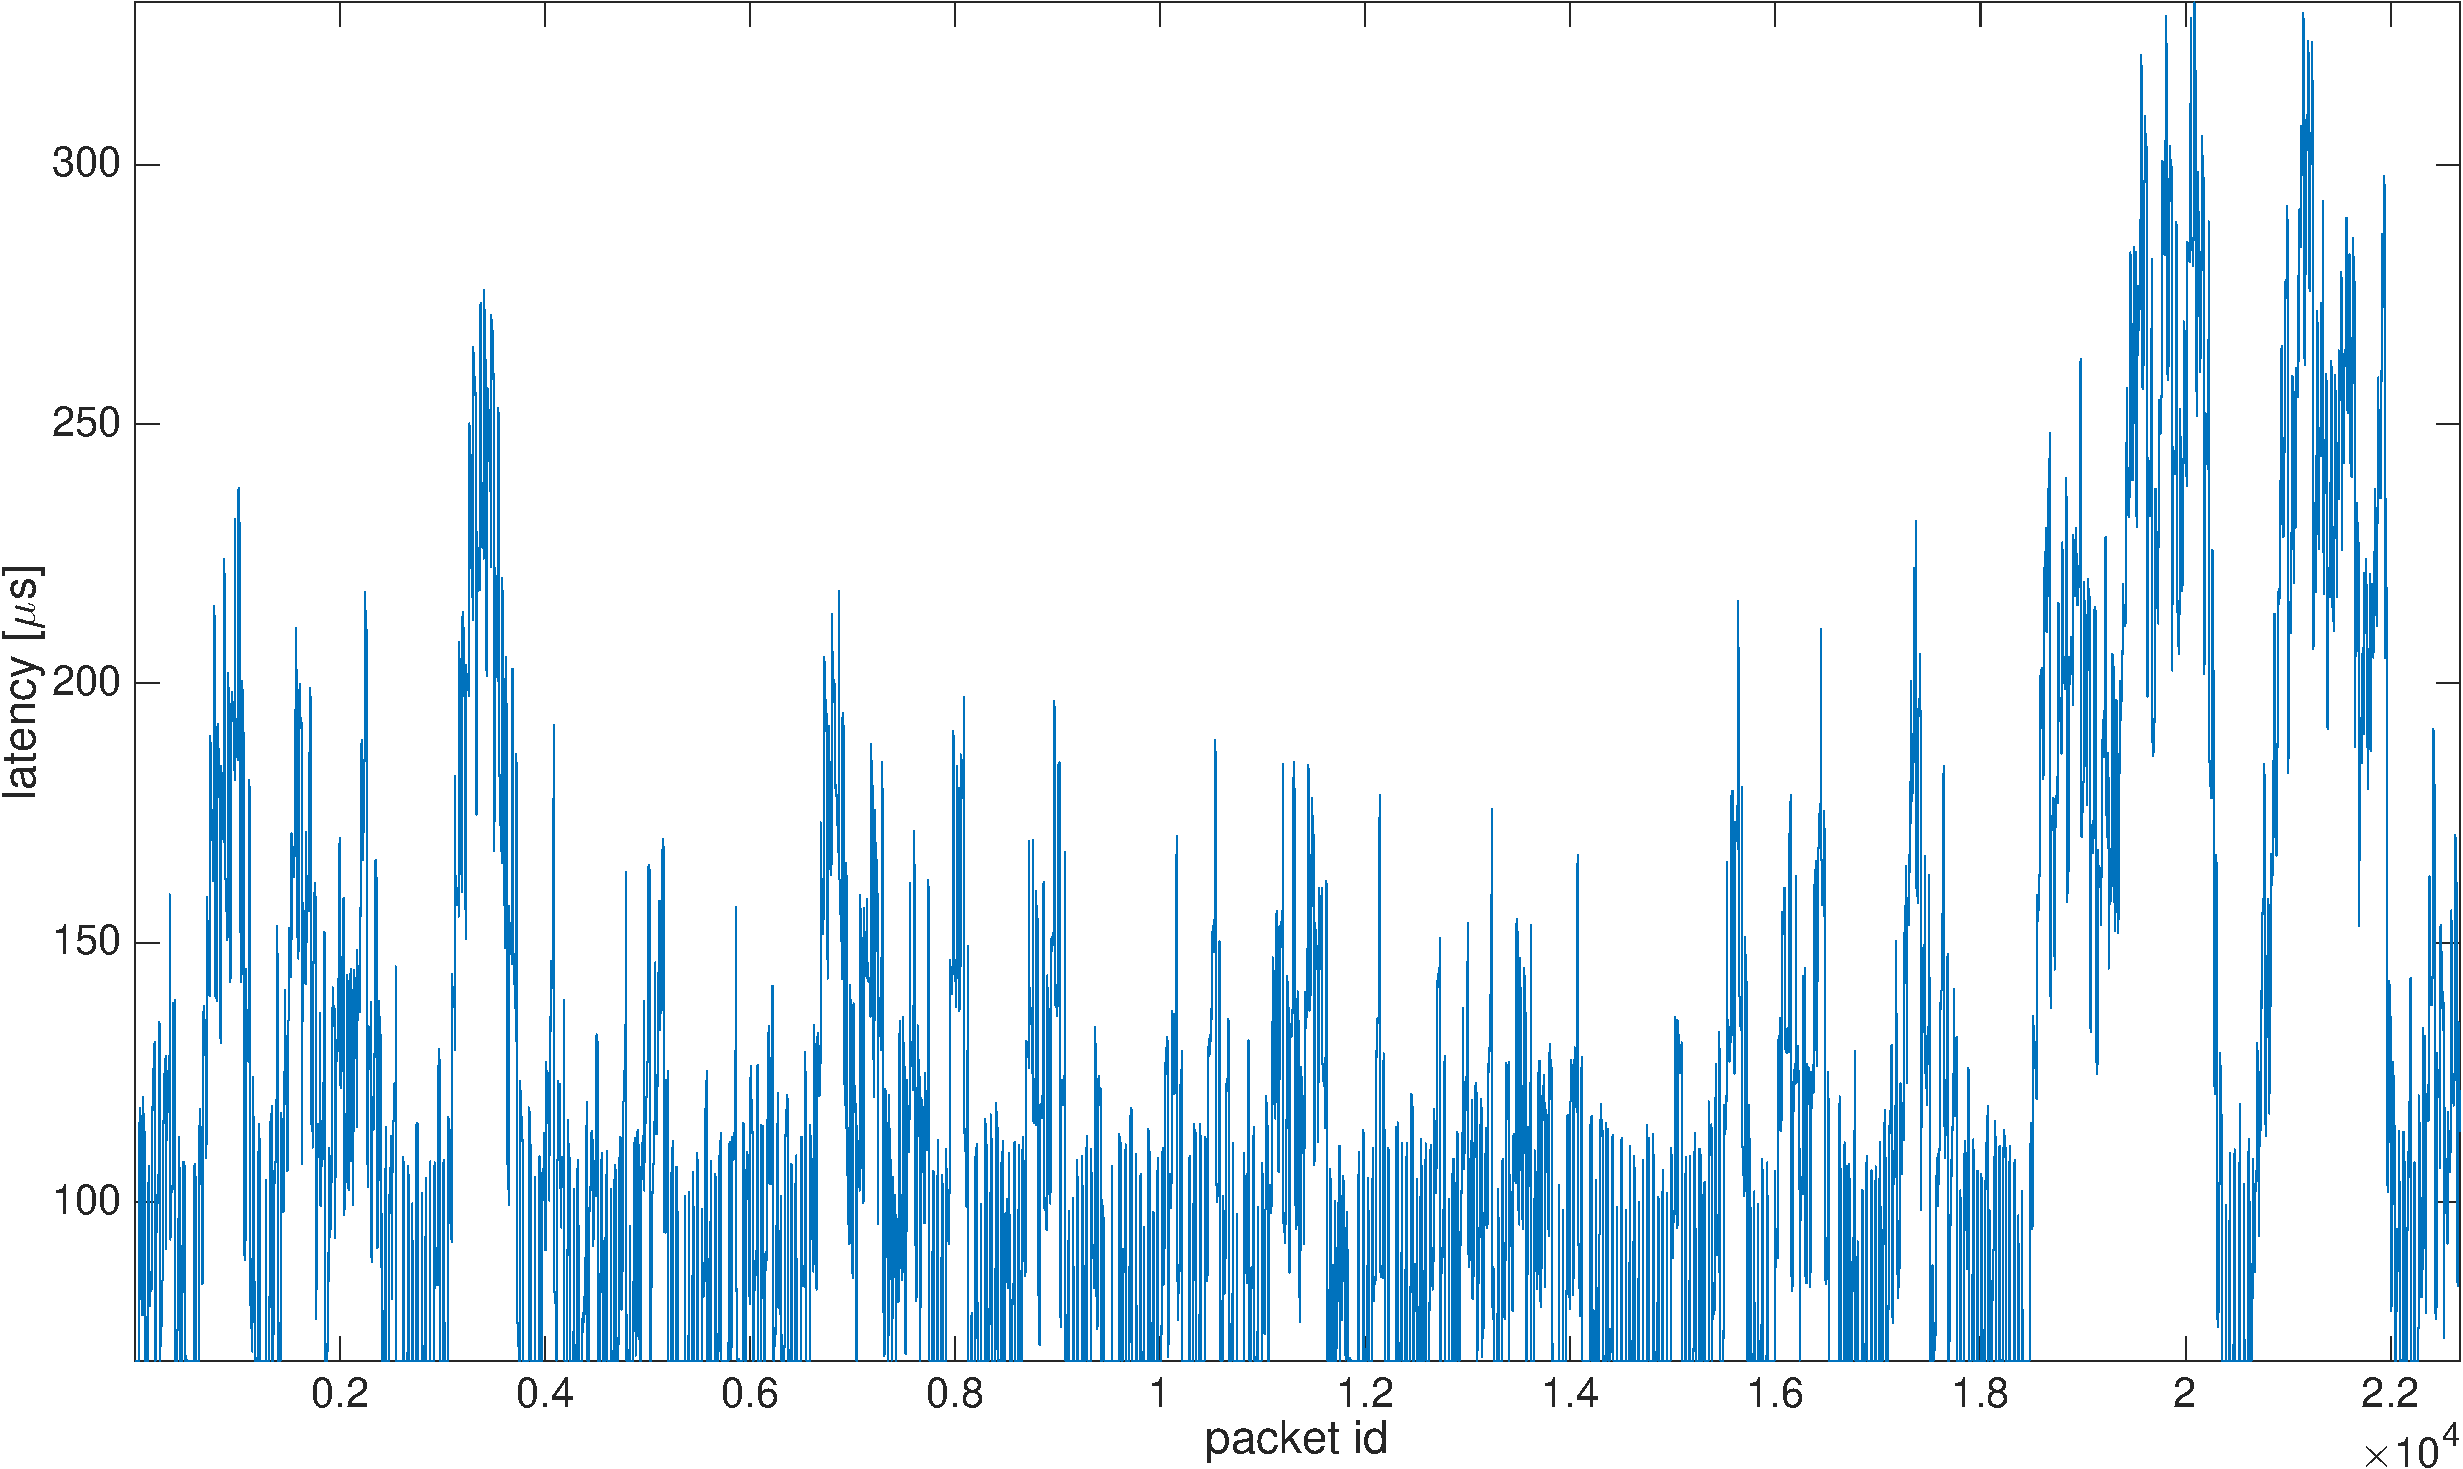
\includegraphics[width=\textwidth]{images/experiment/exp2-app1-no-coremask-latency.pdf}
    \caption{Latencies of the heavy flow packets, without coremask.}
    \label{fig:exp2-app1-no-coremask-latency}
  \end{center}
\end{figure}

\begin{figure}[]
  \begin{center}
    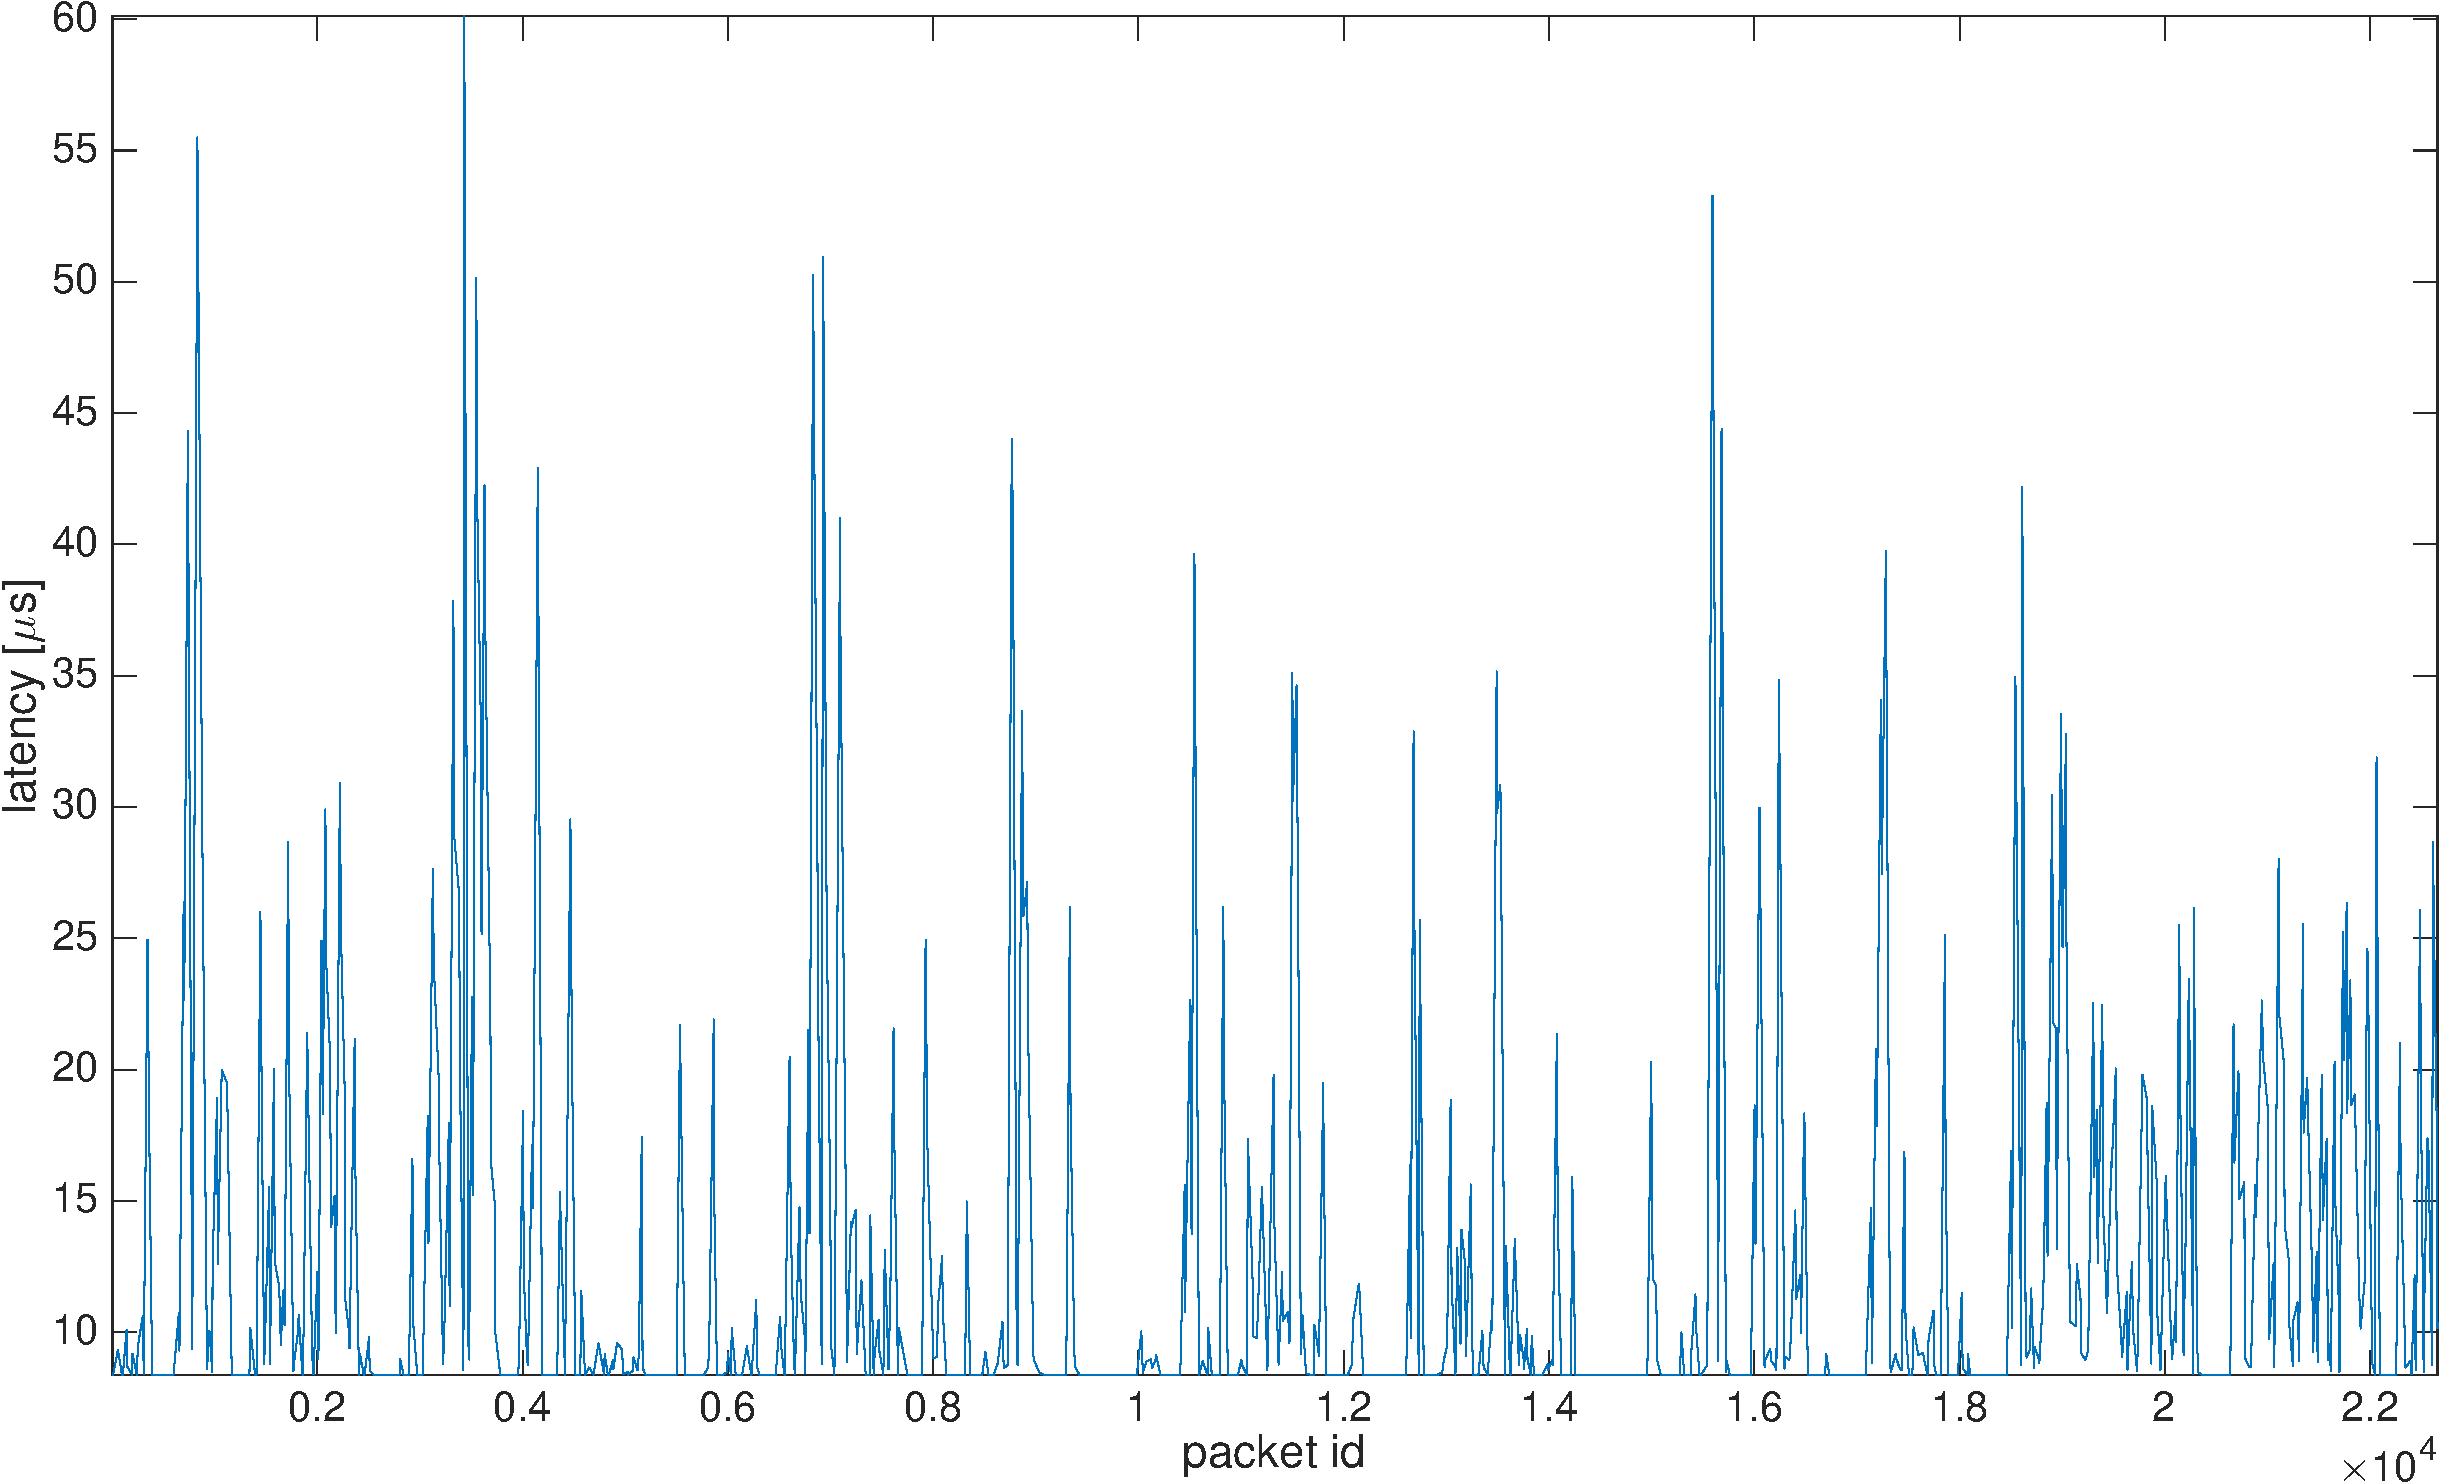
\includegraphics[width=\textwidth]{images/experiment/exp2-app2-no-coremask-latency.pdf}
    \caption{Latencies of the light flow packets, without coremask. The worst case latencies are almost ten-fold compared to the best case.}
    \label{fig:exp2-app2-no-coremask-latency}
  \end{center}
\end{figure}

In the second simulation, we use a modified coremask for the heavy application, i.e. dedicating one of the cores for the light application processing. The resulting latencies of the heavy and light flow are presented in figures~\ref{fig:exp2-app1-is-coremask-latency} and~\ref{fig:exp2-app2-is-coremask-latency}, respectively.

As the figures show, the light flow's worst-case packet latencies can be reduced to less than 12$\mu$s. The throughput of the heavy application is 0.212GBps, corresponding to only 2\% drop compared to the non-coremask processing.

\begin{figure}[]
  \begin{center}
    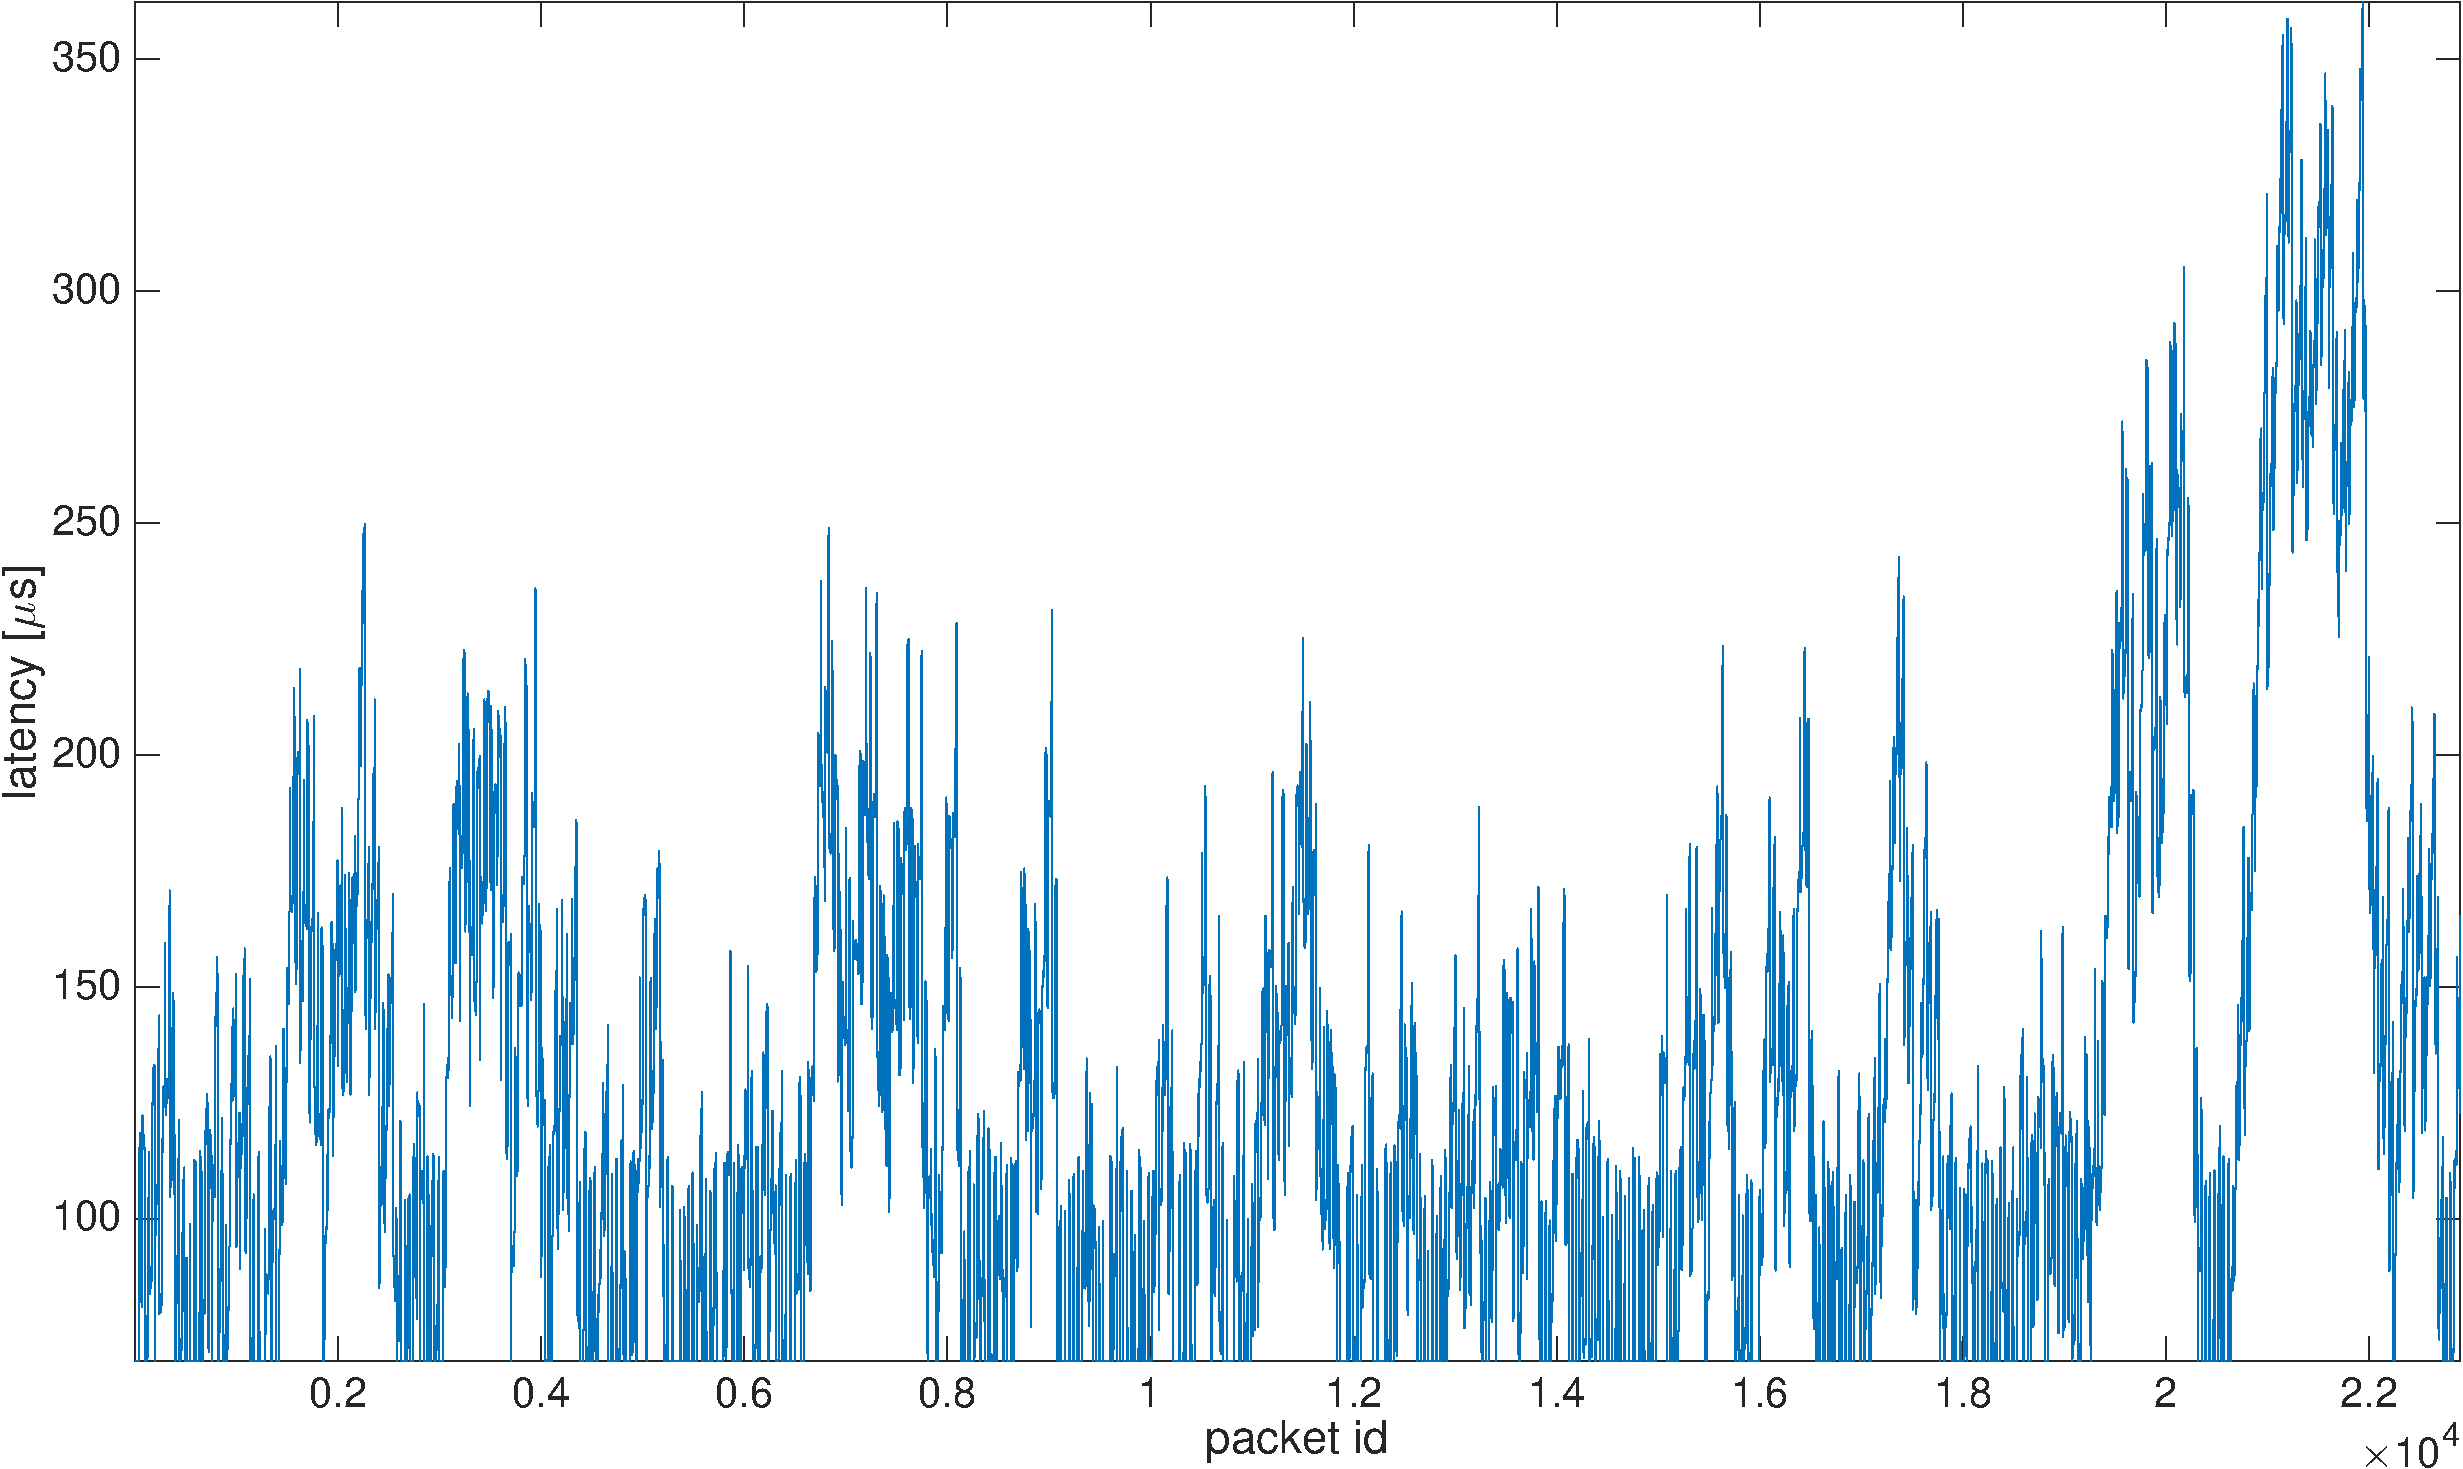
\includegraphics[width=\textwidth]{images/experiment/exp2-app1-is-coremask-latency.pdf}
    \caption{Latencies of the heavy flow packets. One of the cores is dedicated for the light flow.}
    \label{fig:exp2-app1-is-coremask-latency}
  \end{center}
\end{figure}

\begin{figure}[]
  \begin{center}
    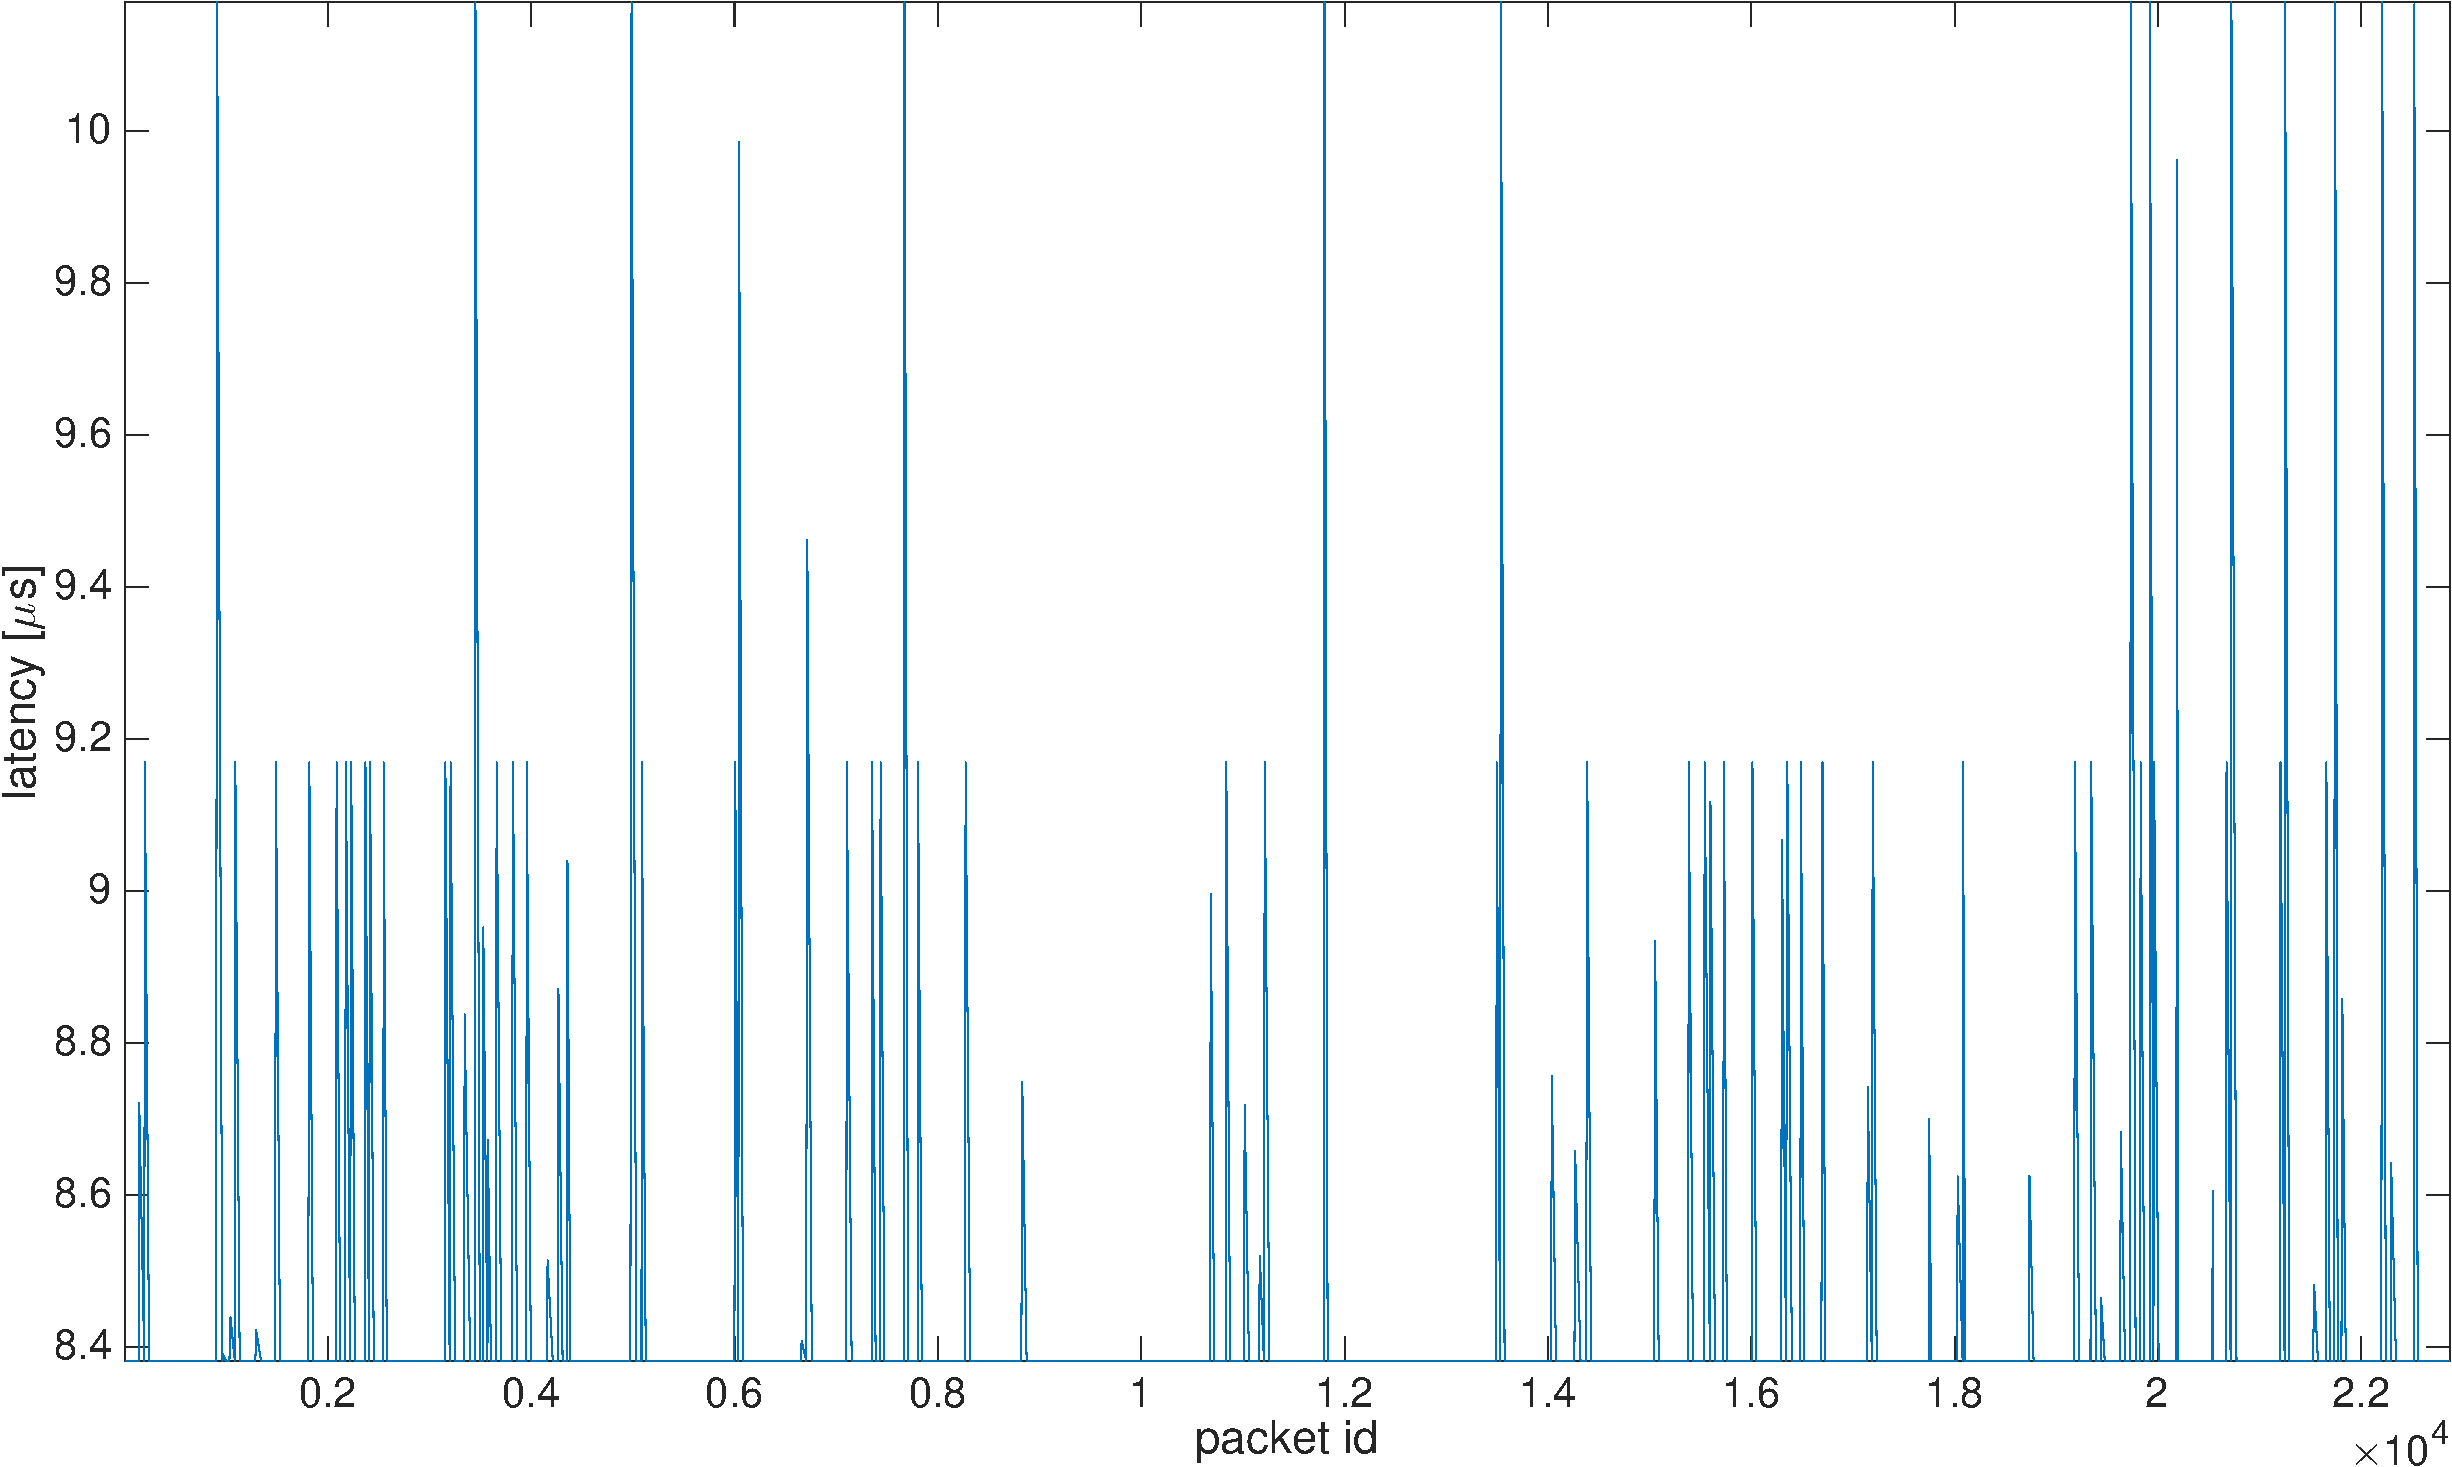
\includegraphics[width=\textwidth]{images/experiment/exp2-app2-is-coremask-latency.pdf}
    \caption{Latencies of the light flow packets. One of the cores is dedicated for the light flow. The worst-case latencies are less than 50\% higher than of the best case.}
    \label{fig:exp2-app2-is-coremask-latency}
  \end{center}
\end{figure}

\section{Discoveries}
The experiments present a proof of concept of the PSE's plugin code mechanism, and the model of Cavium OCTEON II CN6880 network processing unit. The simulation results are encouraging. In both experiments, the model acts as expected. According to the experiment results, the PSE's plugin mechanism seems to be a viable tool for modeling complex hardware and software co-scheduled manycore systems, such as the CN6880's SSO-unit.

More importantly, the plugin code mechanism extends to any resource network based simulation task, providing flexibility, hopefully allowing even more complex systems to be modeled.

%%% Local Variables:
%%% mode: latex
%%% TeX-master: "thesis-hartikainen"
%%% End:
